
		\begin{figure}
			\centering
			\subfloat[SHREK]{
				\scalebox{.4}{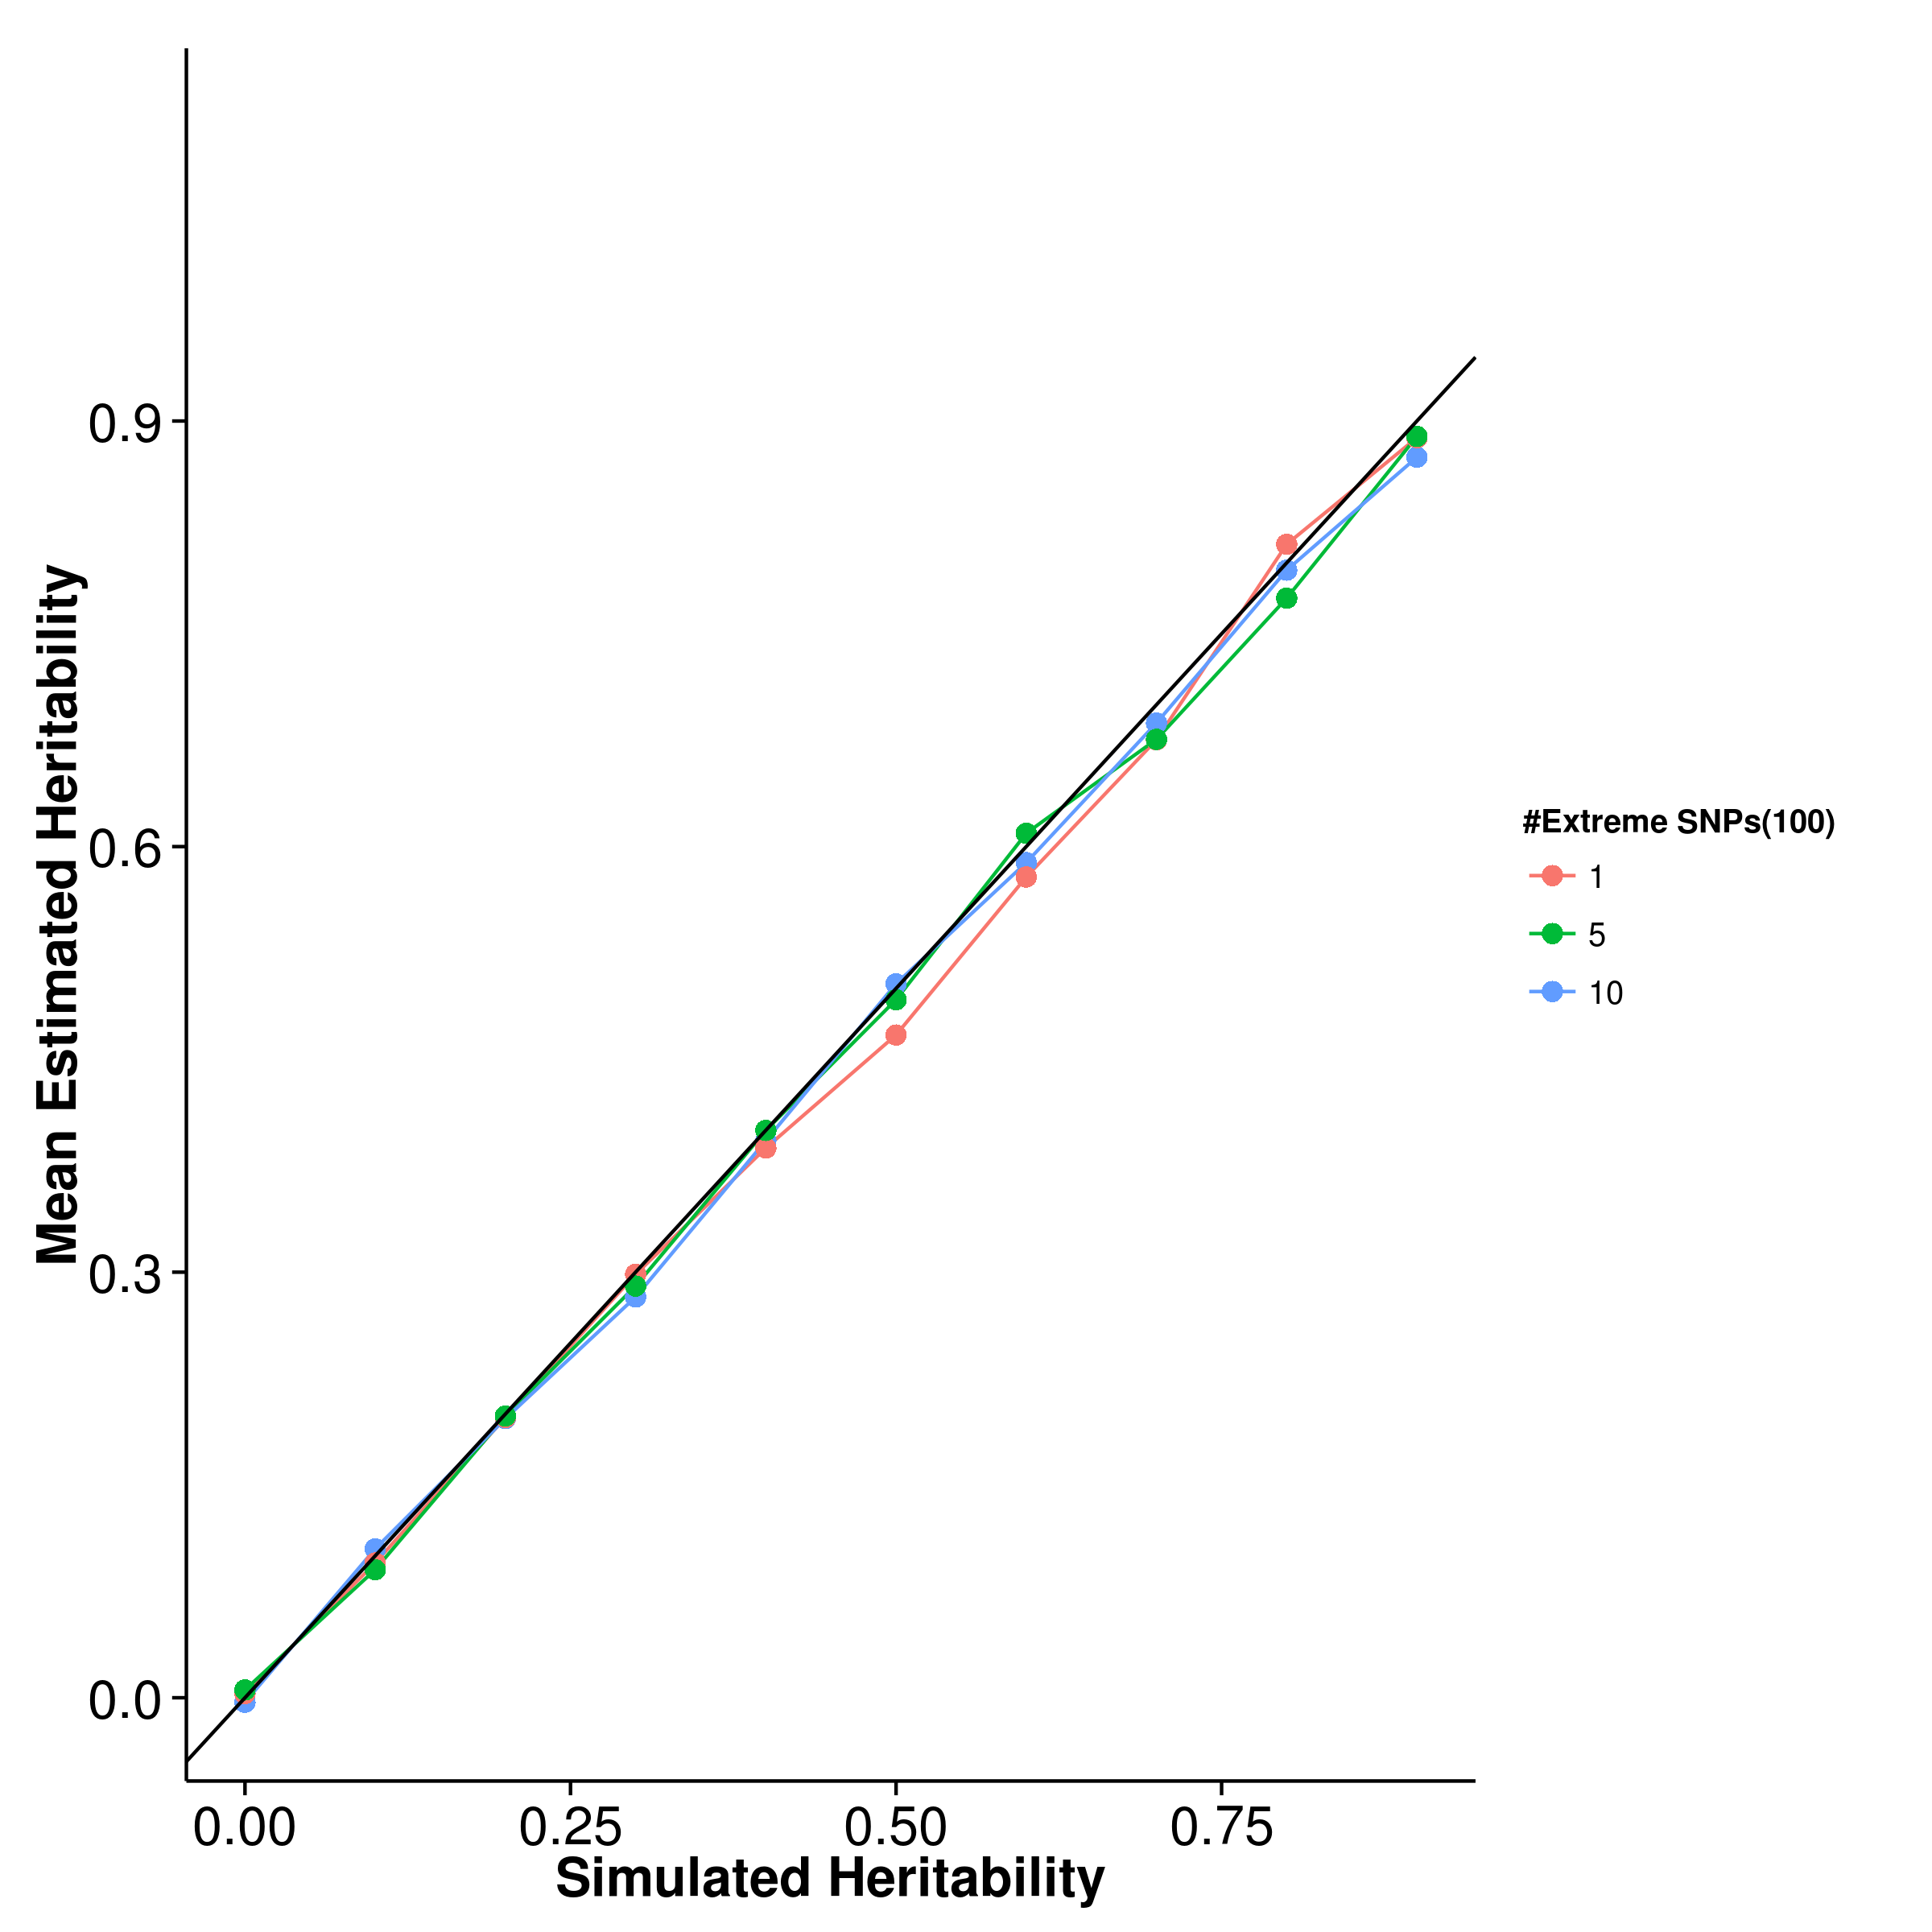
\includegraphics{figure/he_summary/extreme_100c/shrek_QtE_Extreme_mean.png}}
				\label{fig:shrekQtEx100cMean}
			}
			\subfloat[GCTA]{
				\scalebox{.4}{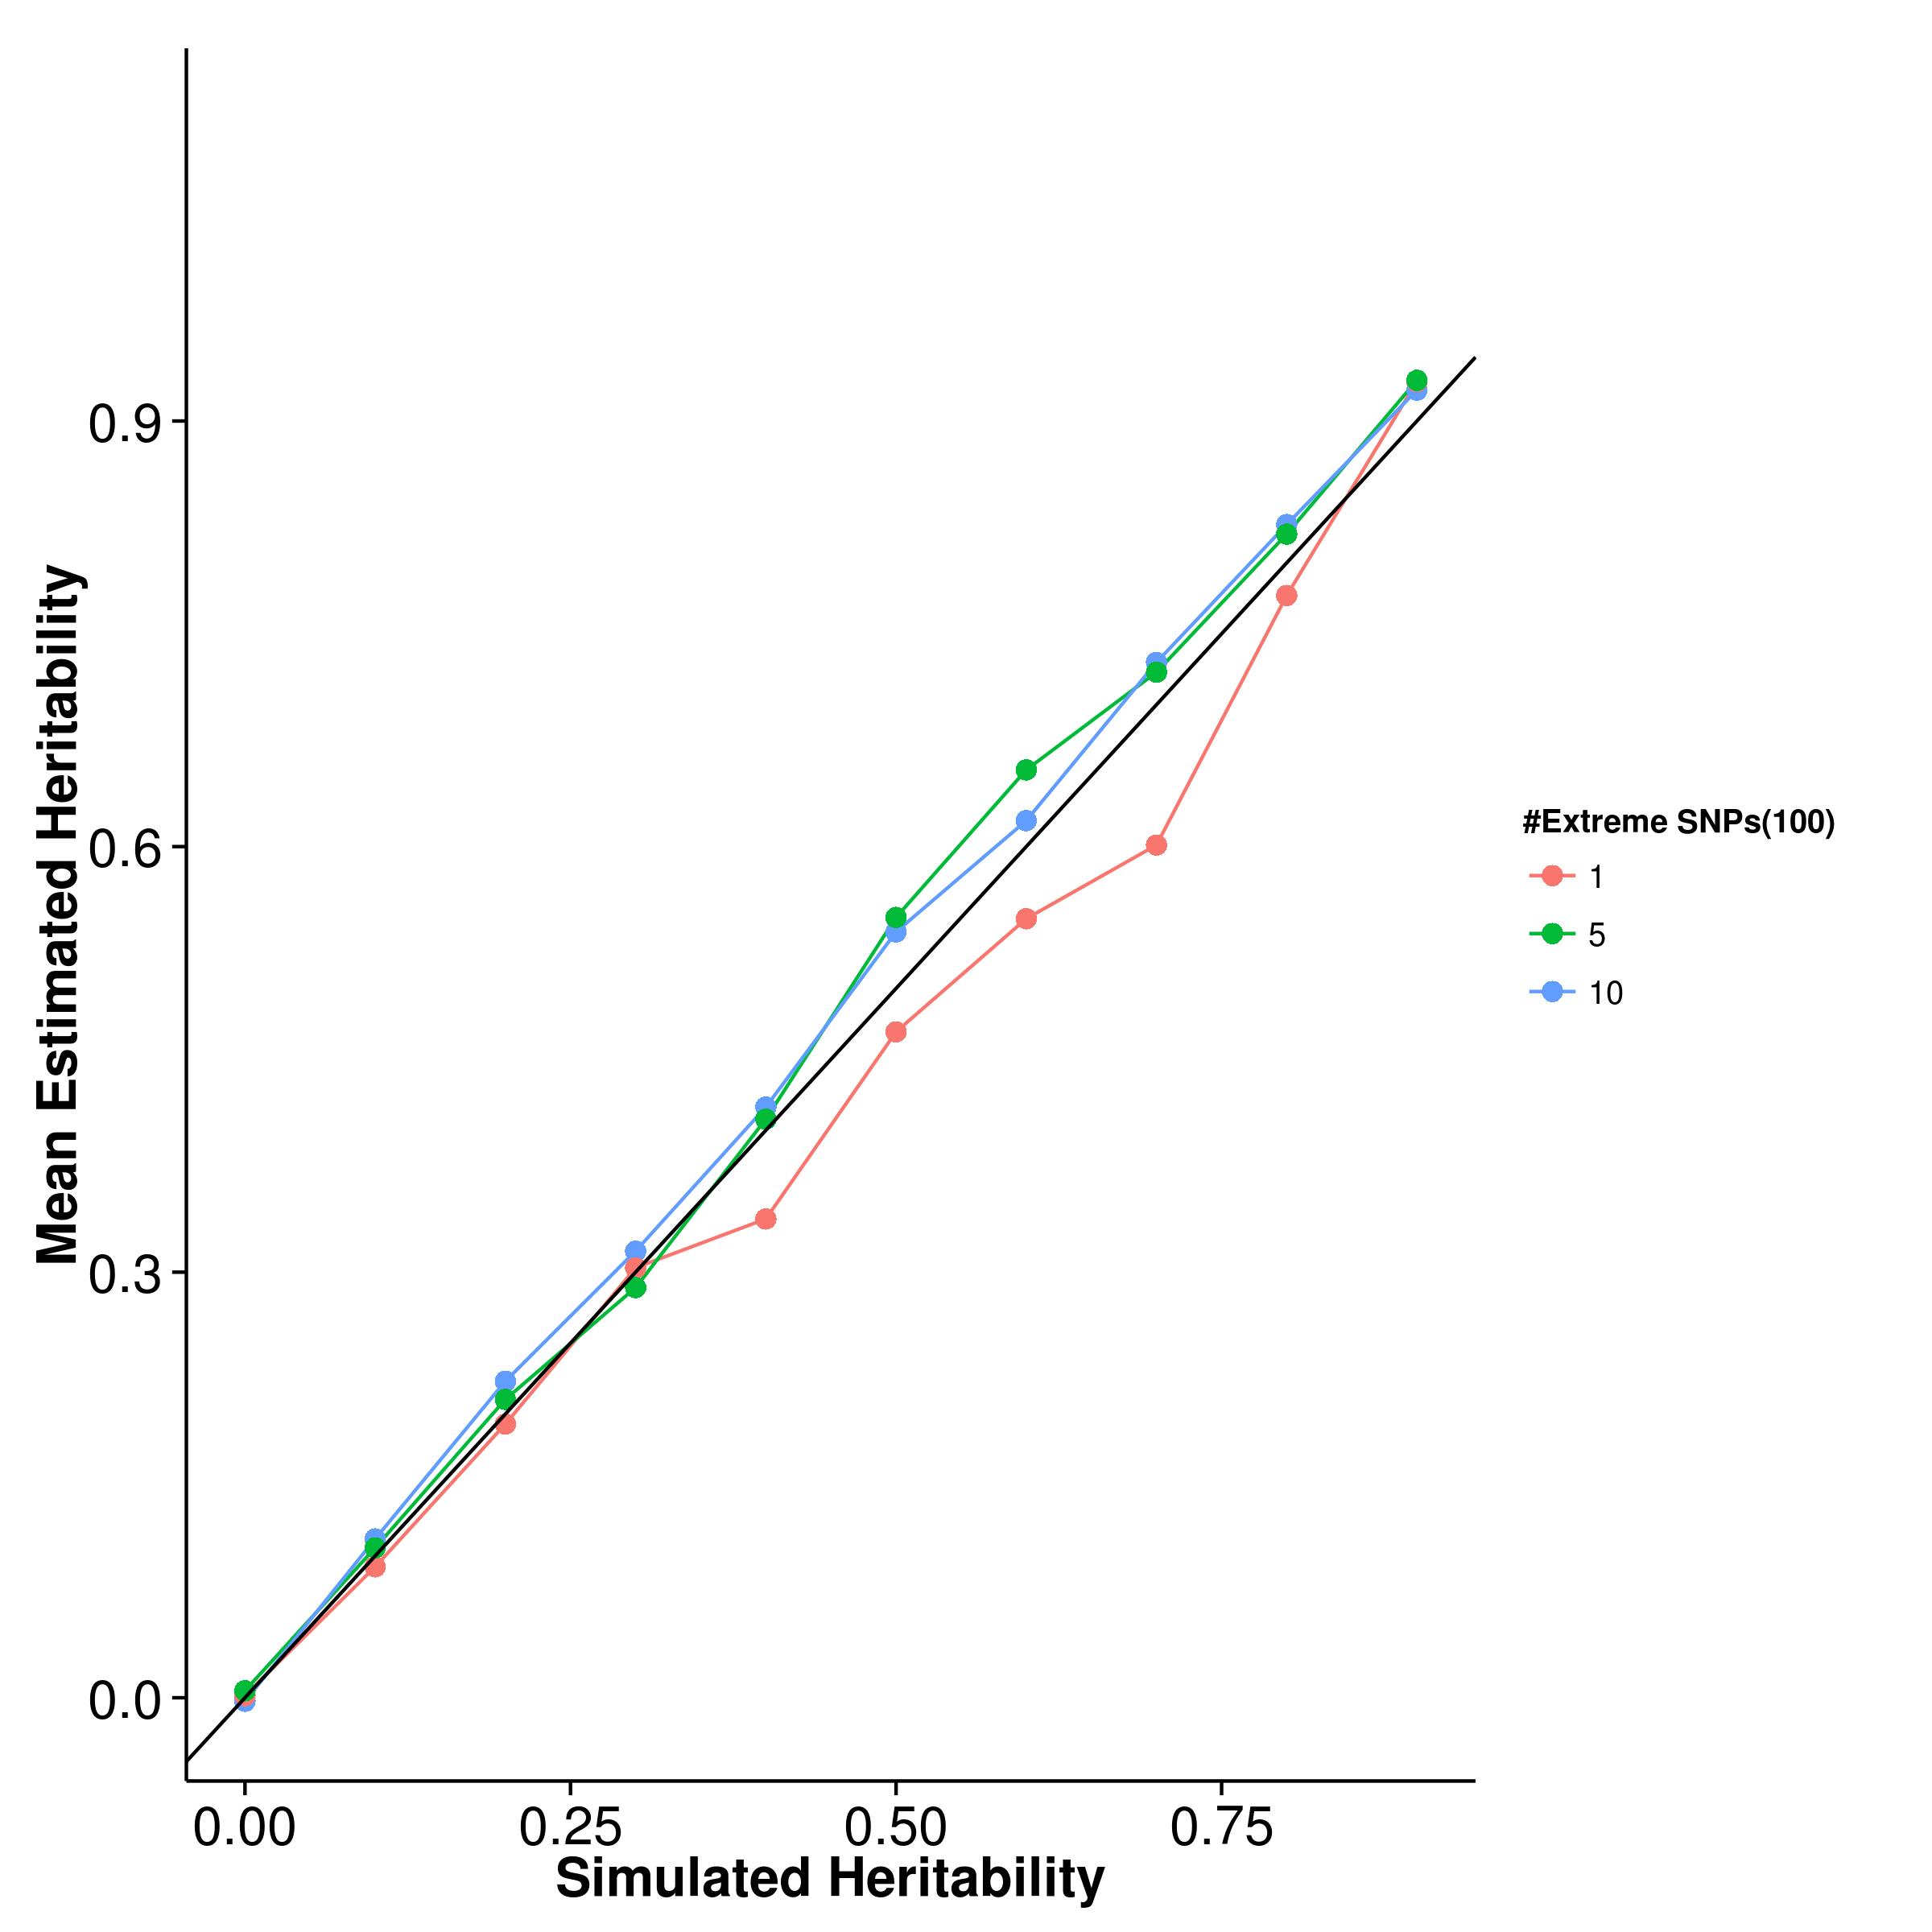
\includegraphics{figure/he_summary/extreme_100c/gcta_QtE_Extreme_mean.png}}
				\label{fig:gctaQtEx100cMean}
			}\\
			\subfloat[LDSC with fix intercept]{
				\scalebox{.4}{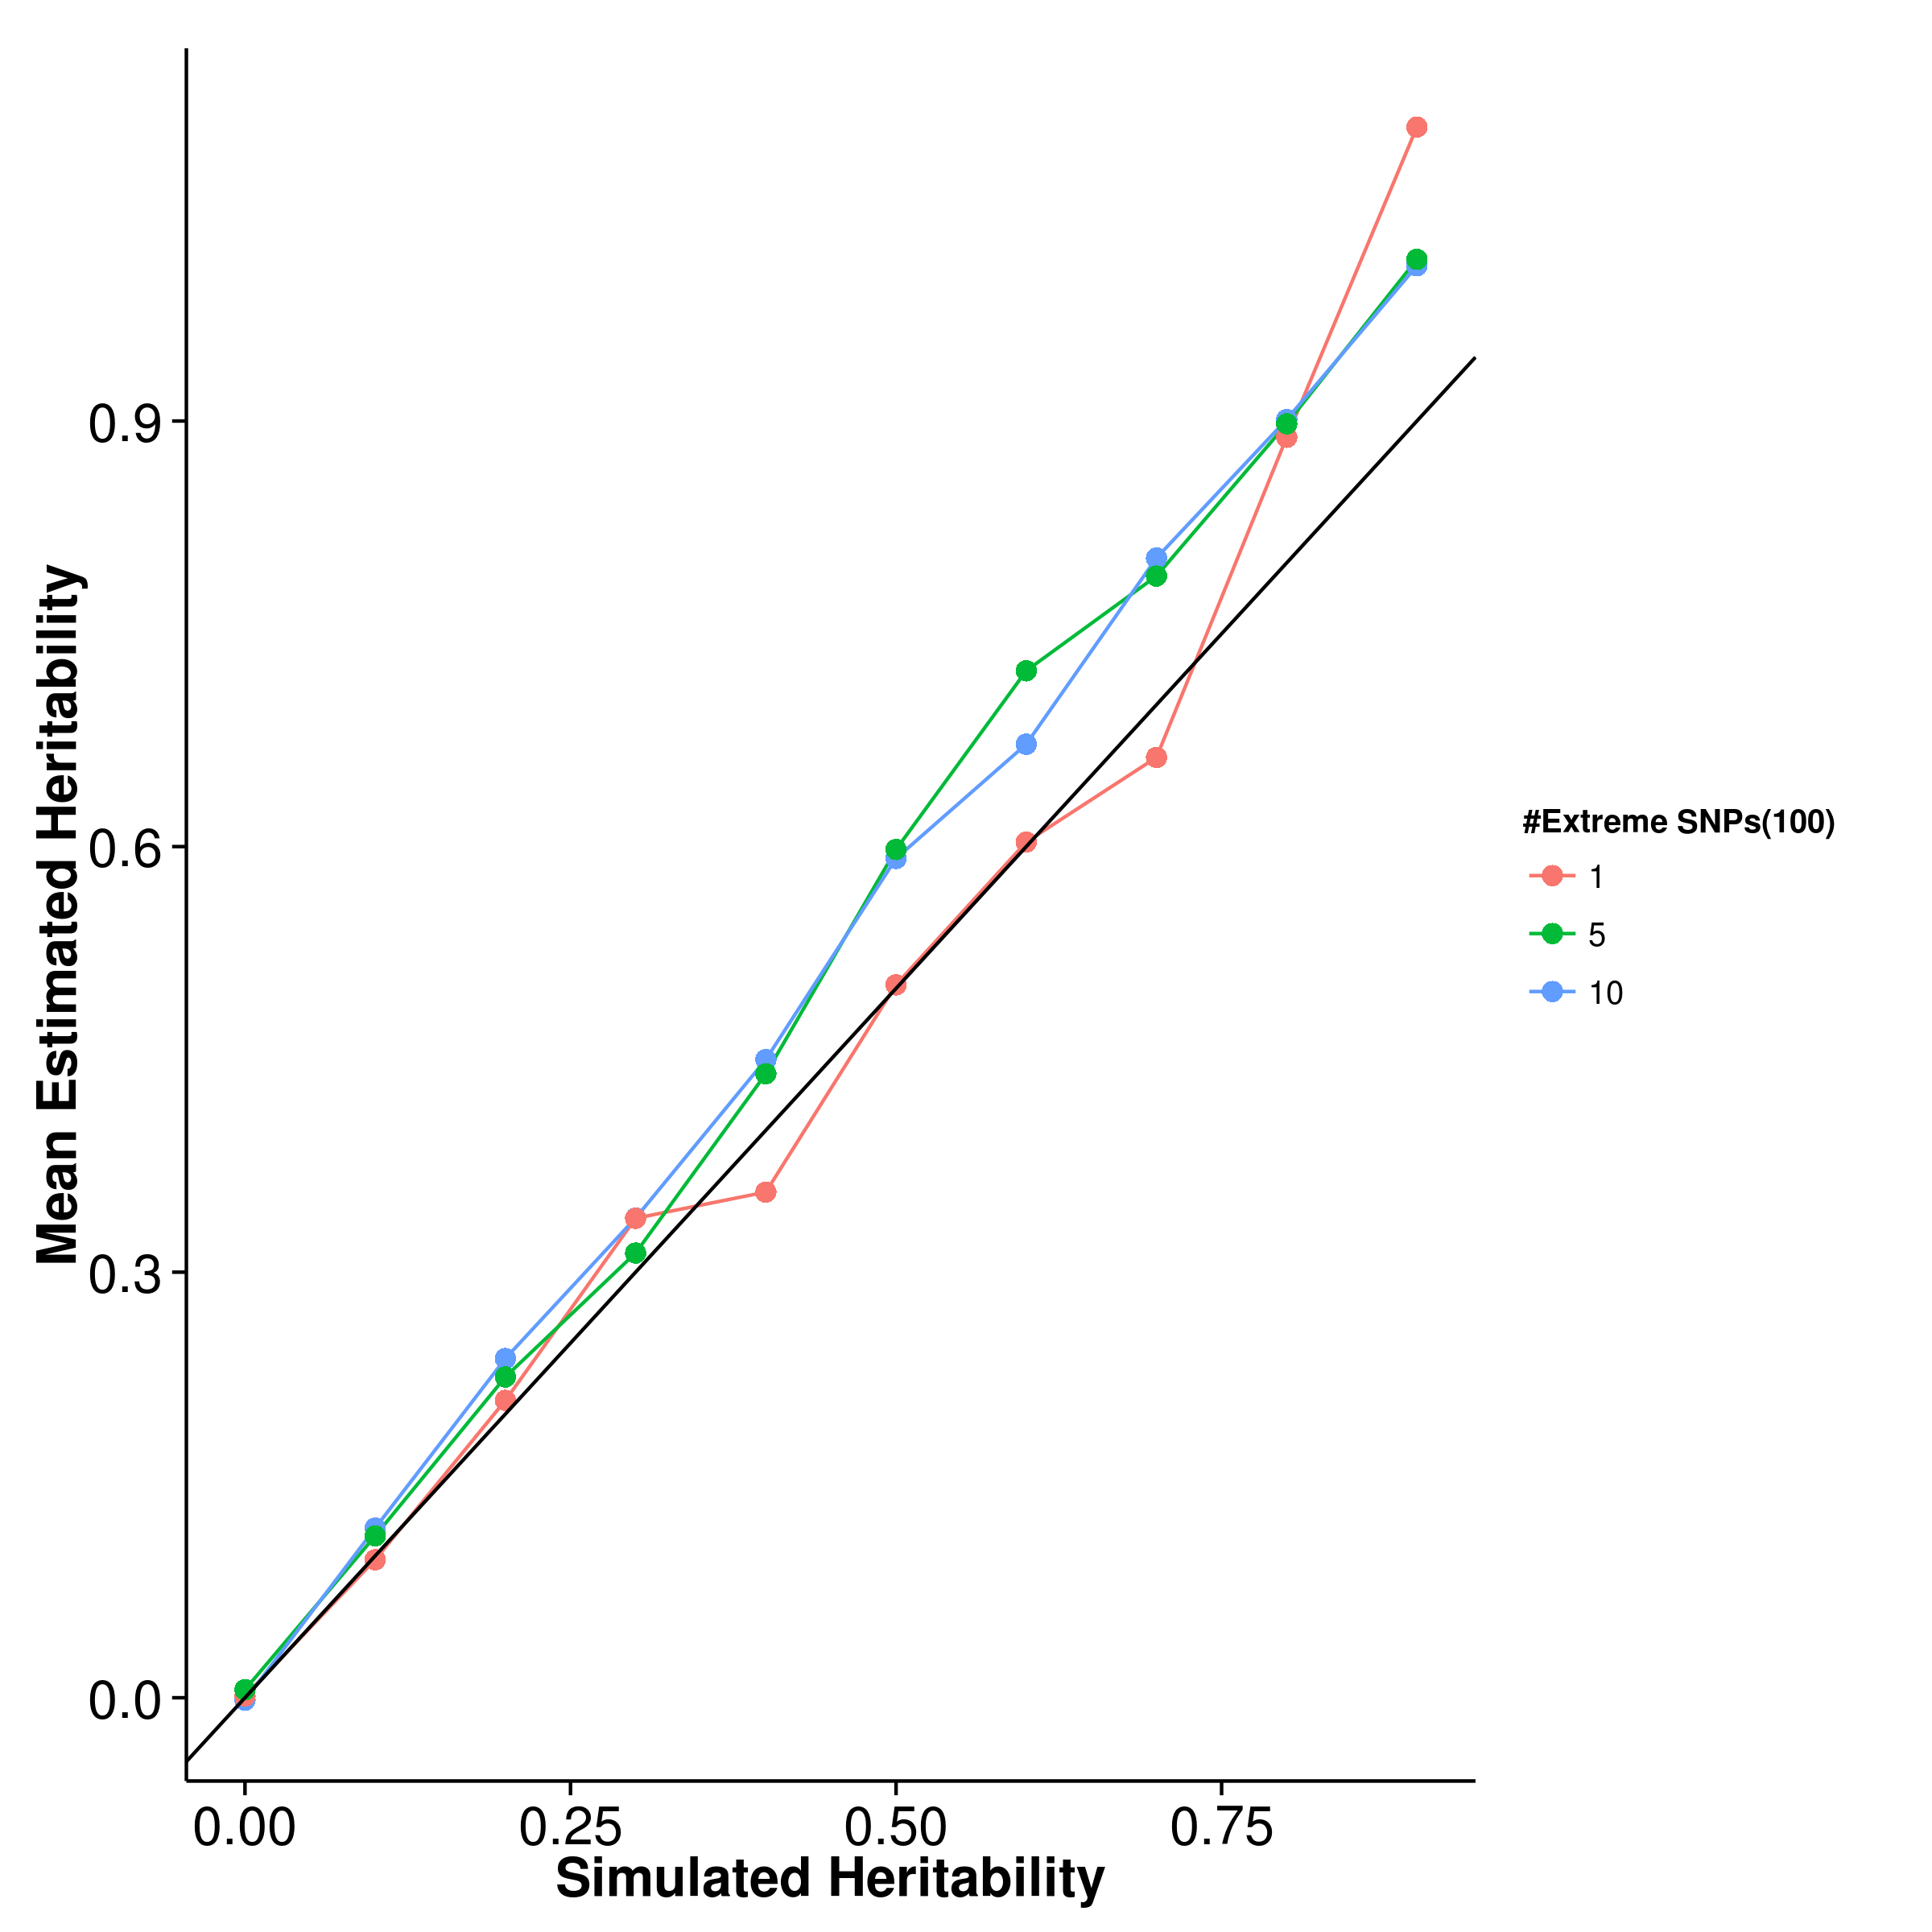
\includegraphics{figure/he_summary/extreme_100c/ldsc_QtE_Extreme_mean.png}}
				\label{fig:ldscQtEx100cMean}
			}
			\subfloat[LDSC with intercept estimation]{
				
				\scalebox{.4}{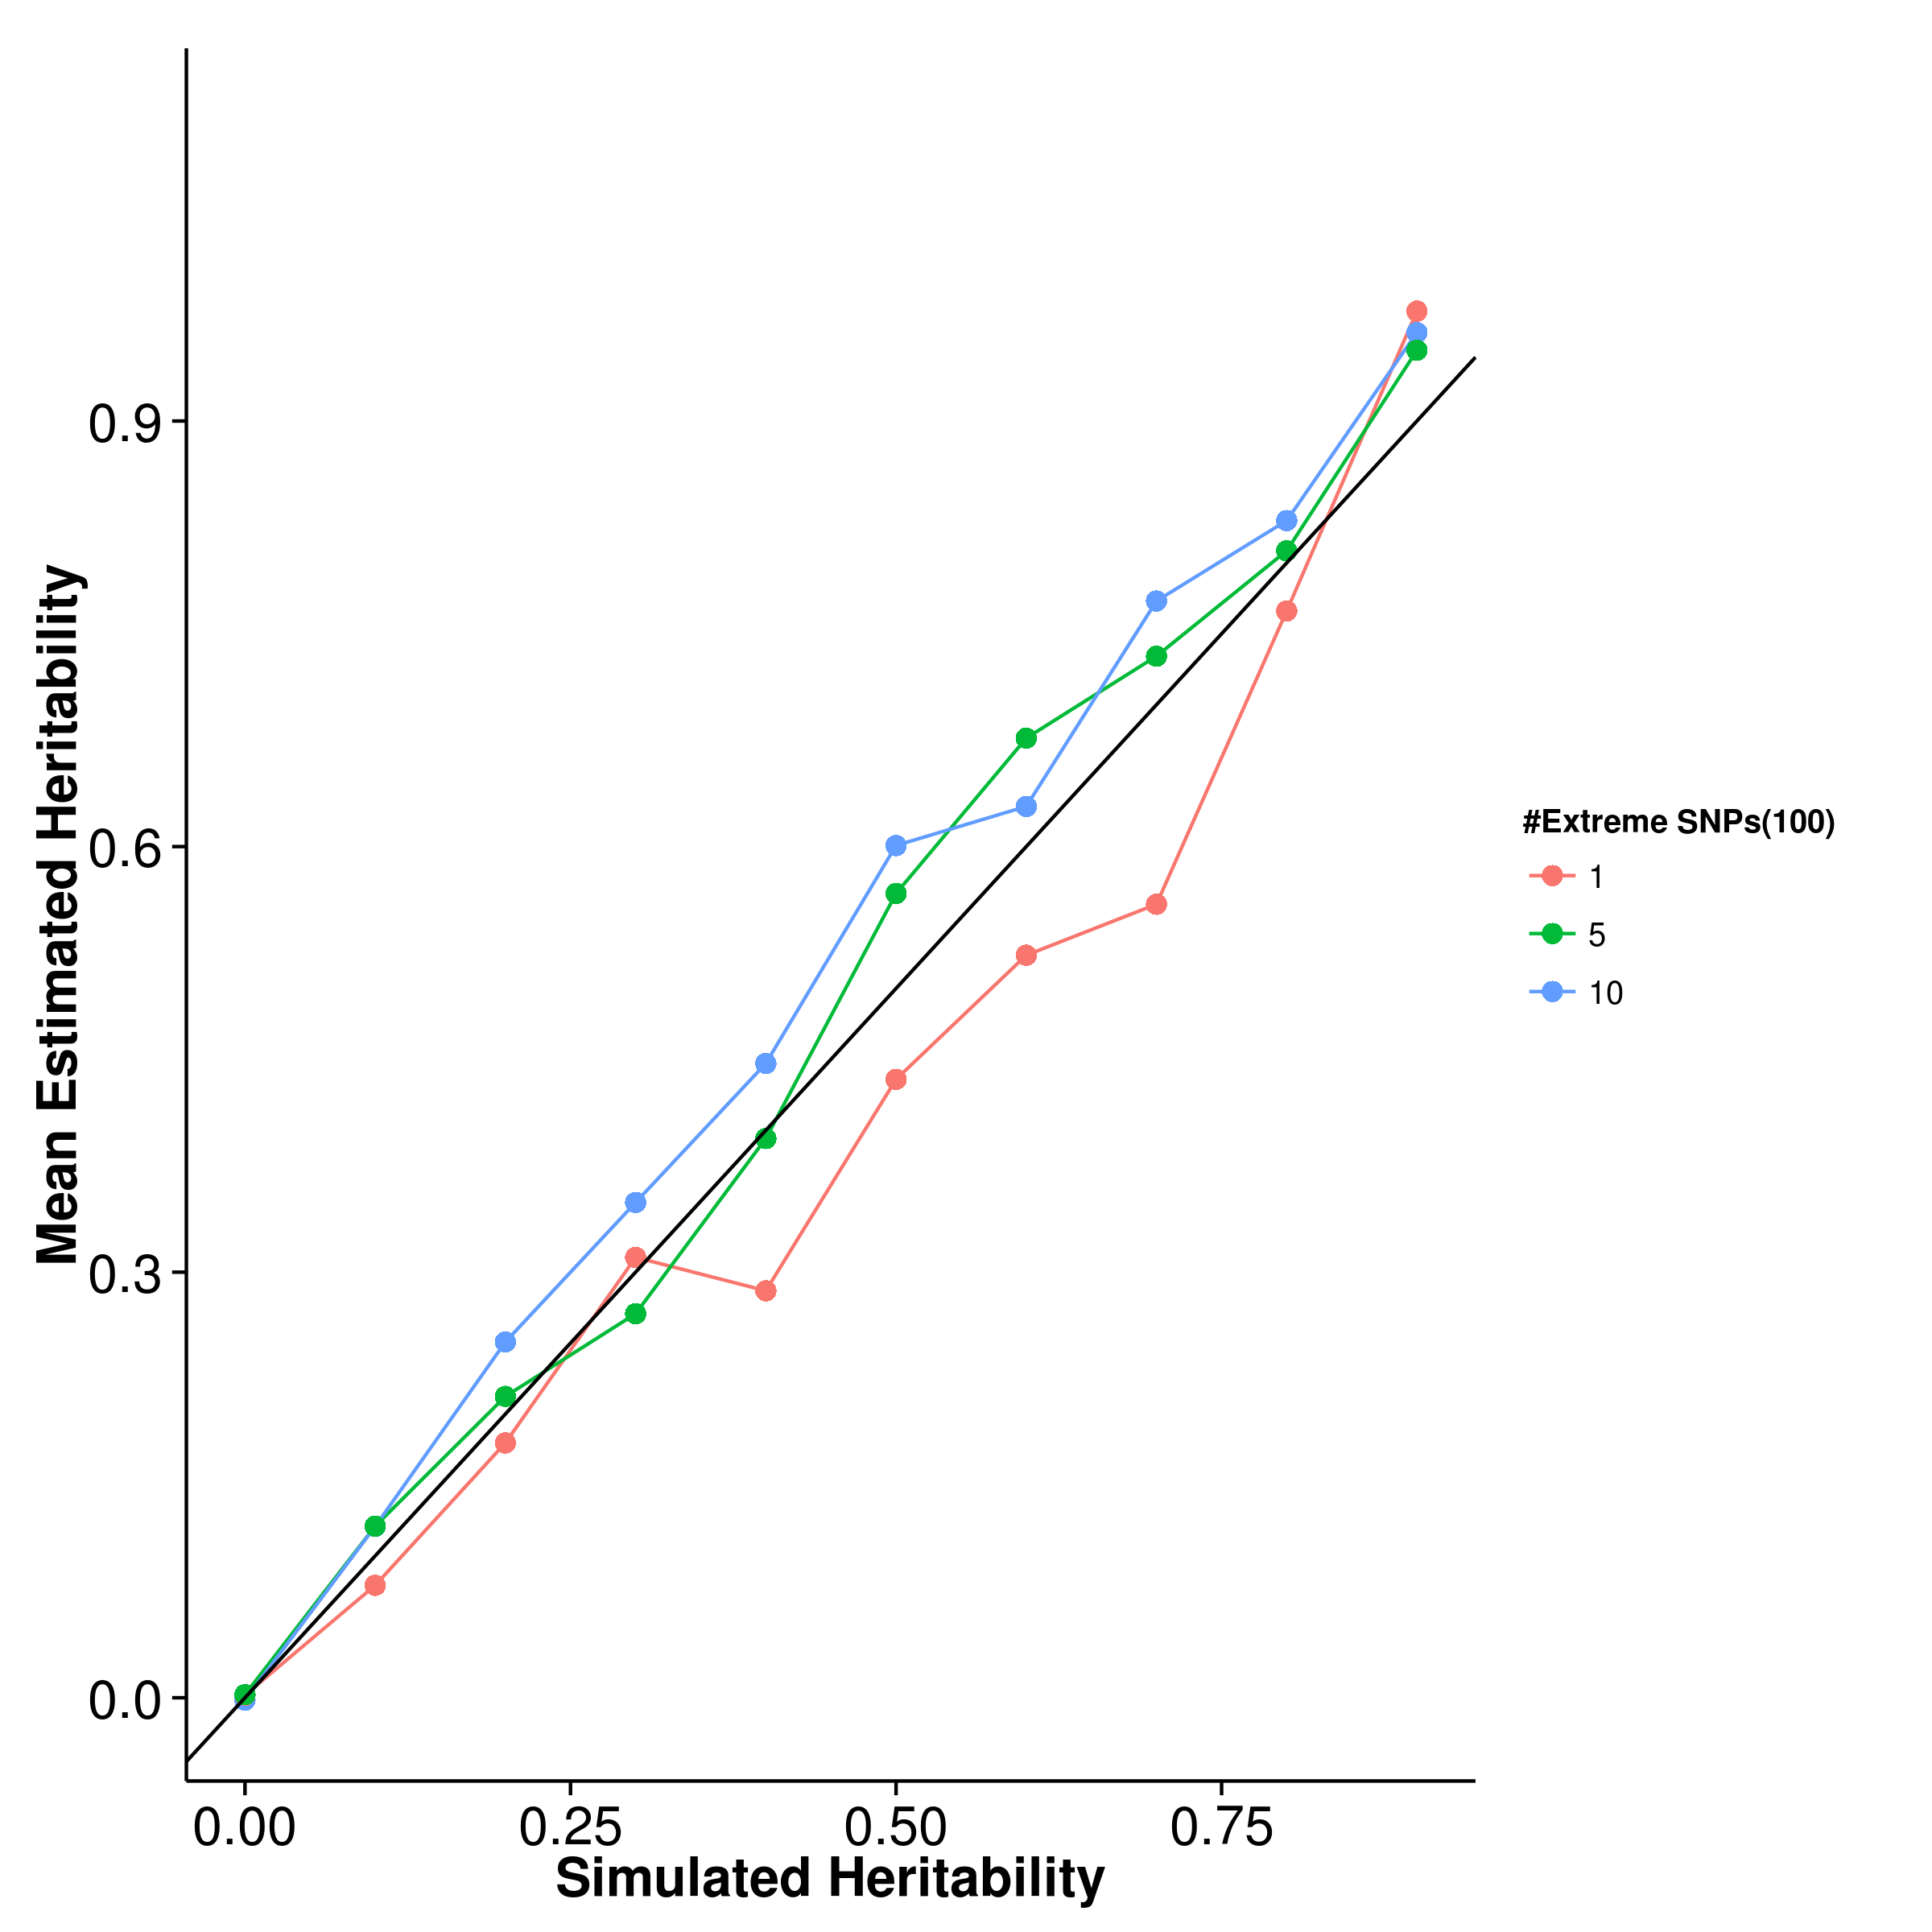
\includegraphics{figure/he_summary/extreme_100c/ldscIn_QtE_Extreme_mean.png}}
				\label{fig:ldscInQtEx100cMean}
			}
			\caption[Quantitative Trait with Extreme Effect Size Simulation Result(100 causal SNPs, Mean)]
			{Mean of results from quantitative trait simulation with extreme effect size simulation.
				100 causal \glspl{SNP} were simulated.
				It was observed that the mean estimation of heritability of all the tools were relatively unaffected by the number of \glspl{SNP} representing a large portion of effect where \gls{shrek} has the least amount of bias.
				} 
			\label{fig:QtEx100cMean}
		\end{figure}
		
		\begin{figure}
			\centering
			\subfloat[SHREK]{
				\scalebox{.4}{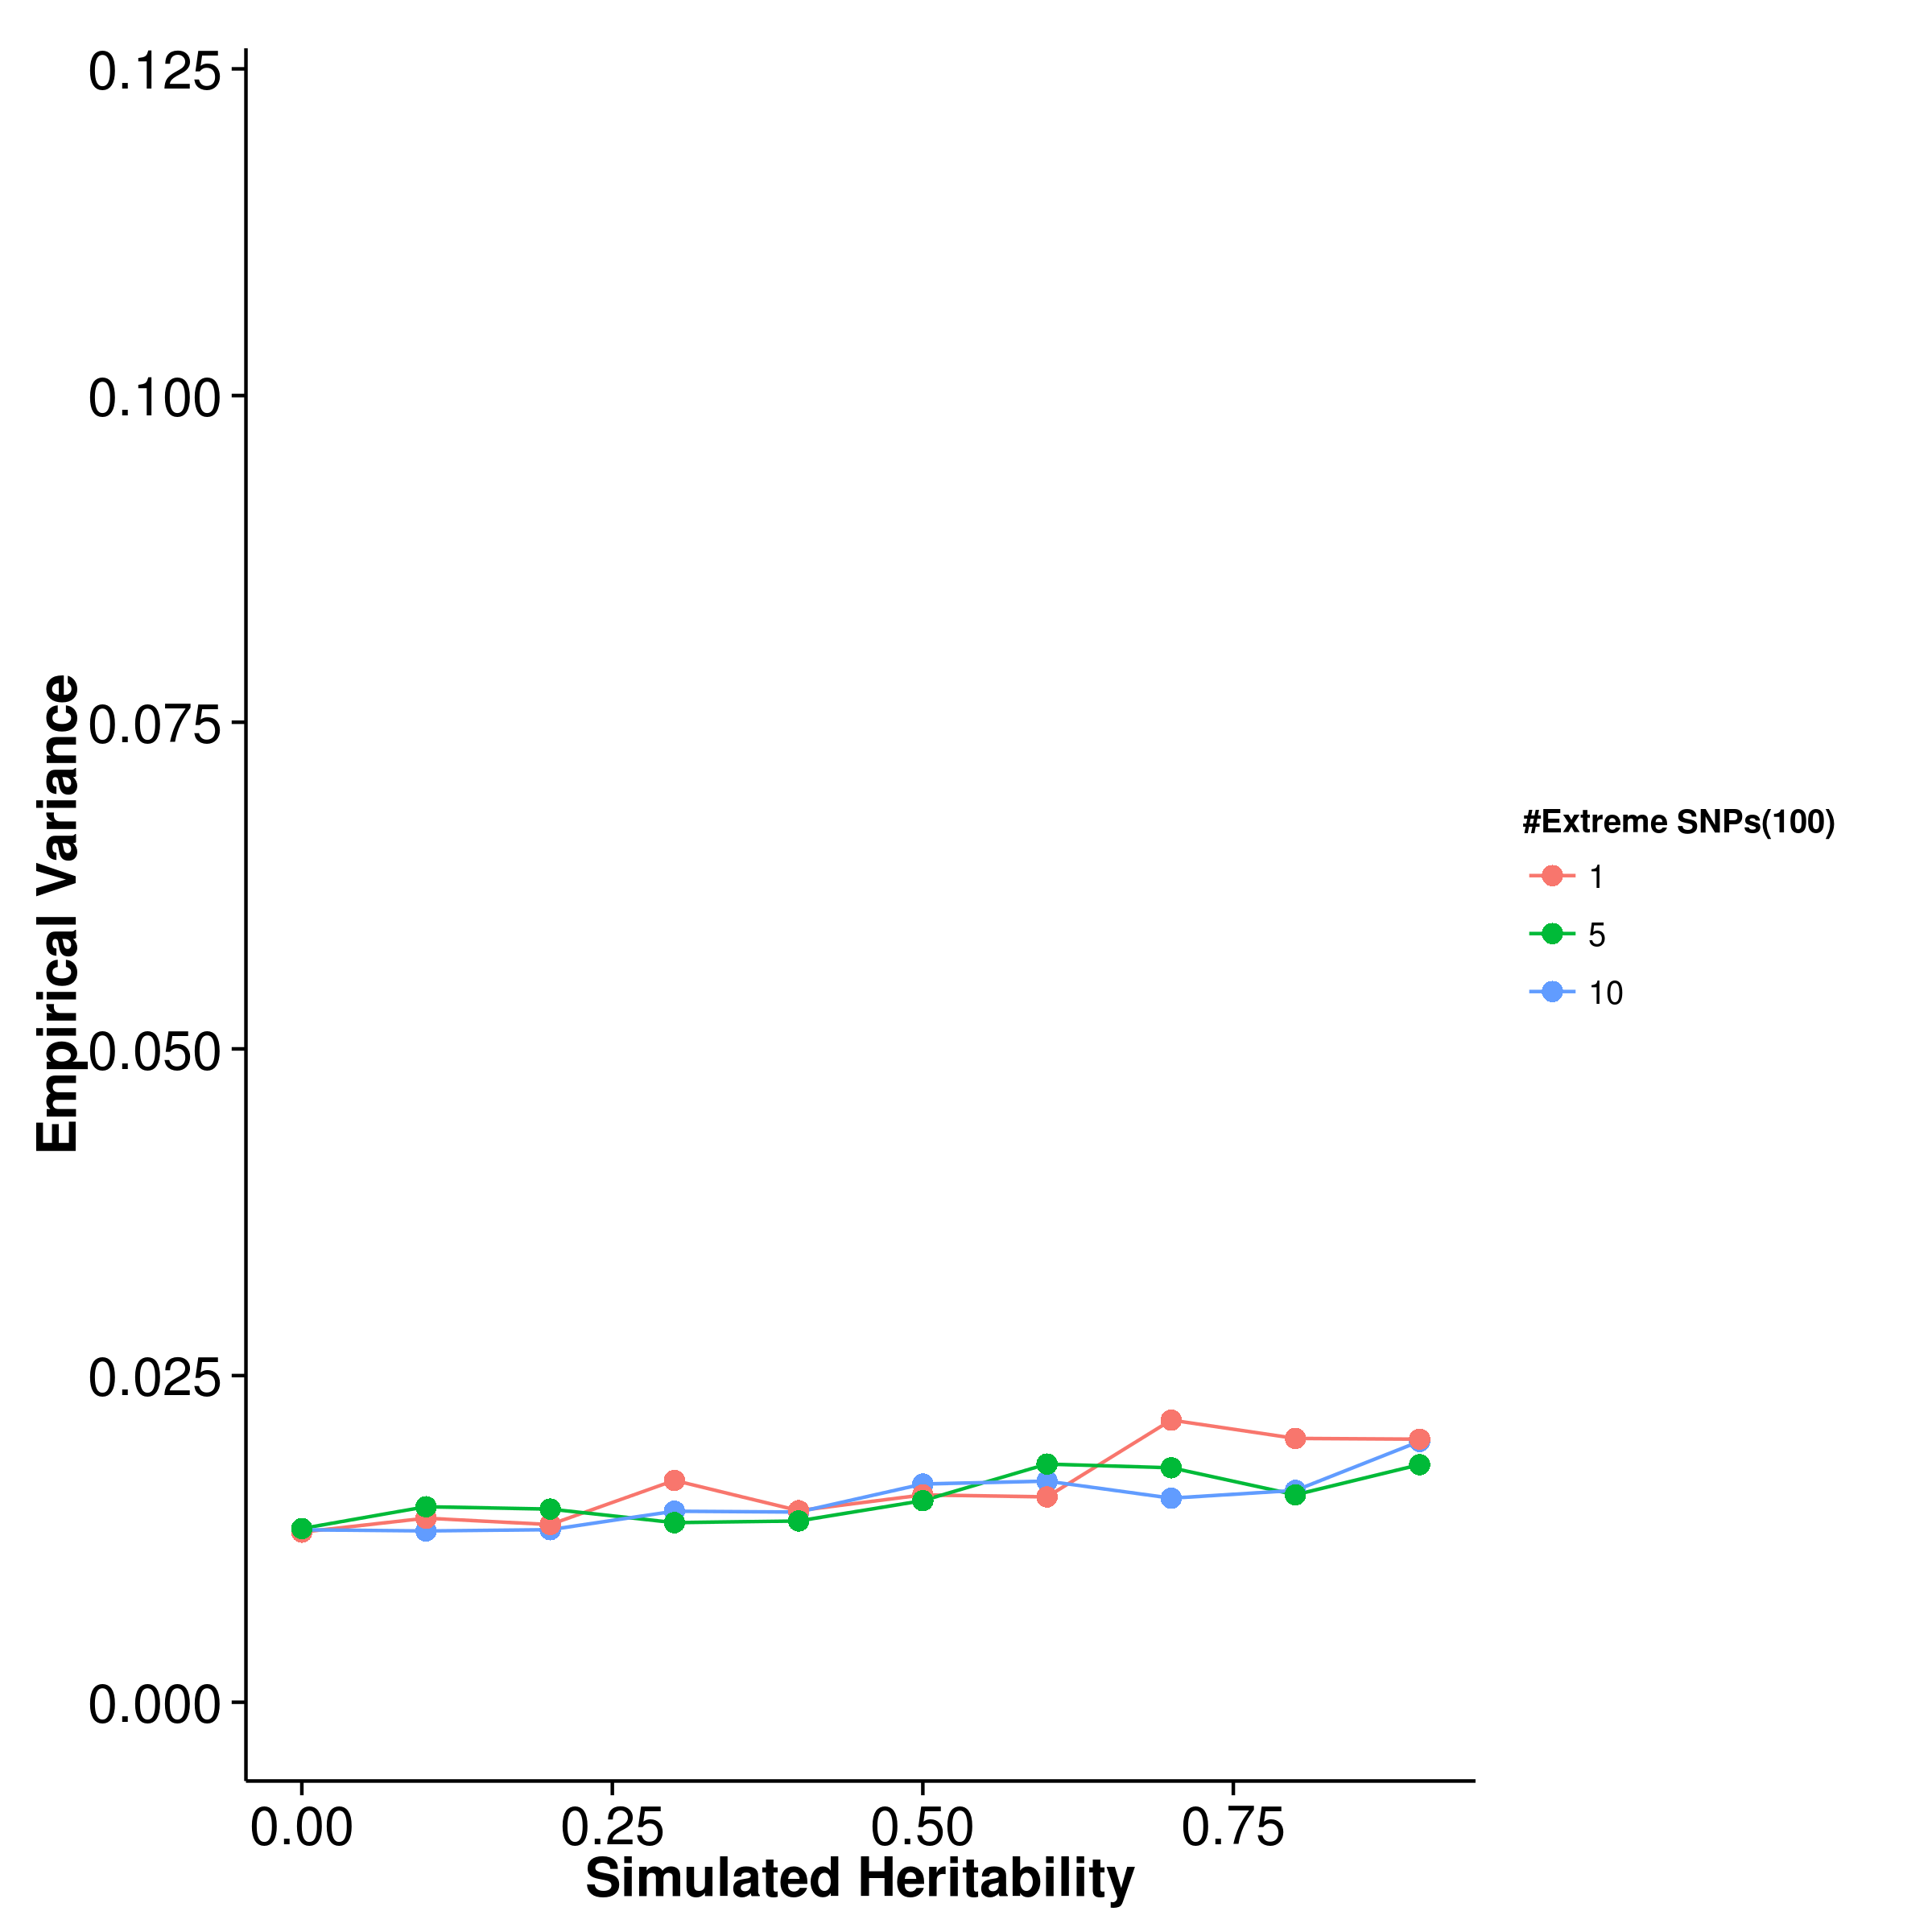
\includegraphics{figure/he_summary/extreme_100c/shrek_QtE_Extreme_sd.png}}
				\label{fig:shrekQtEx100cVar}
			}
			\subfloat[GCTA]{
				\scalebox{.4}{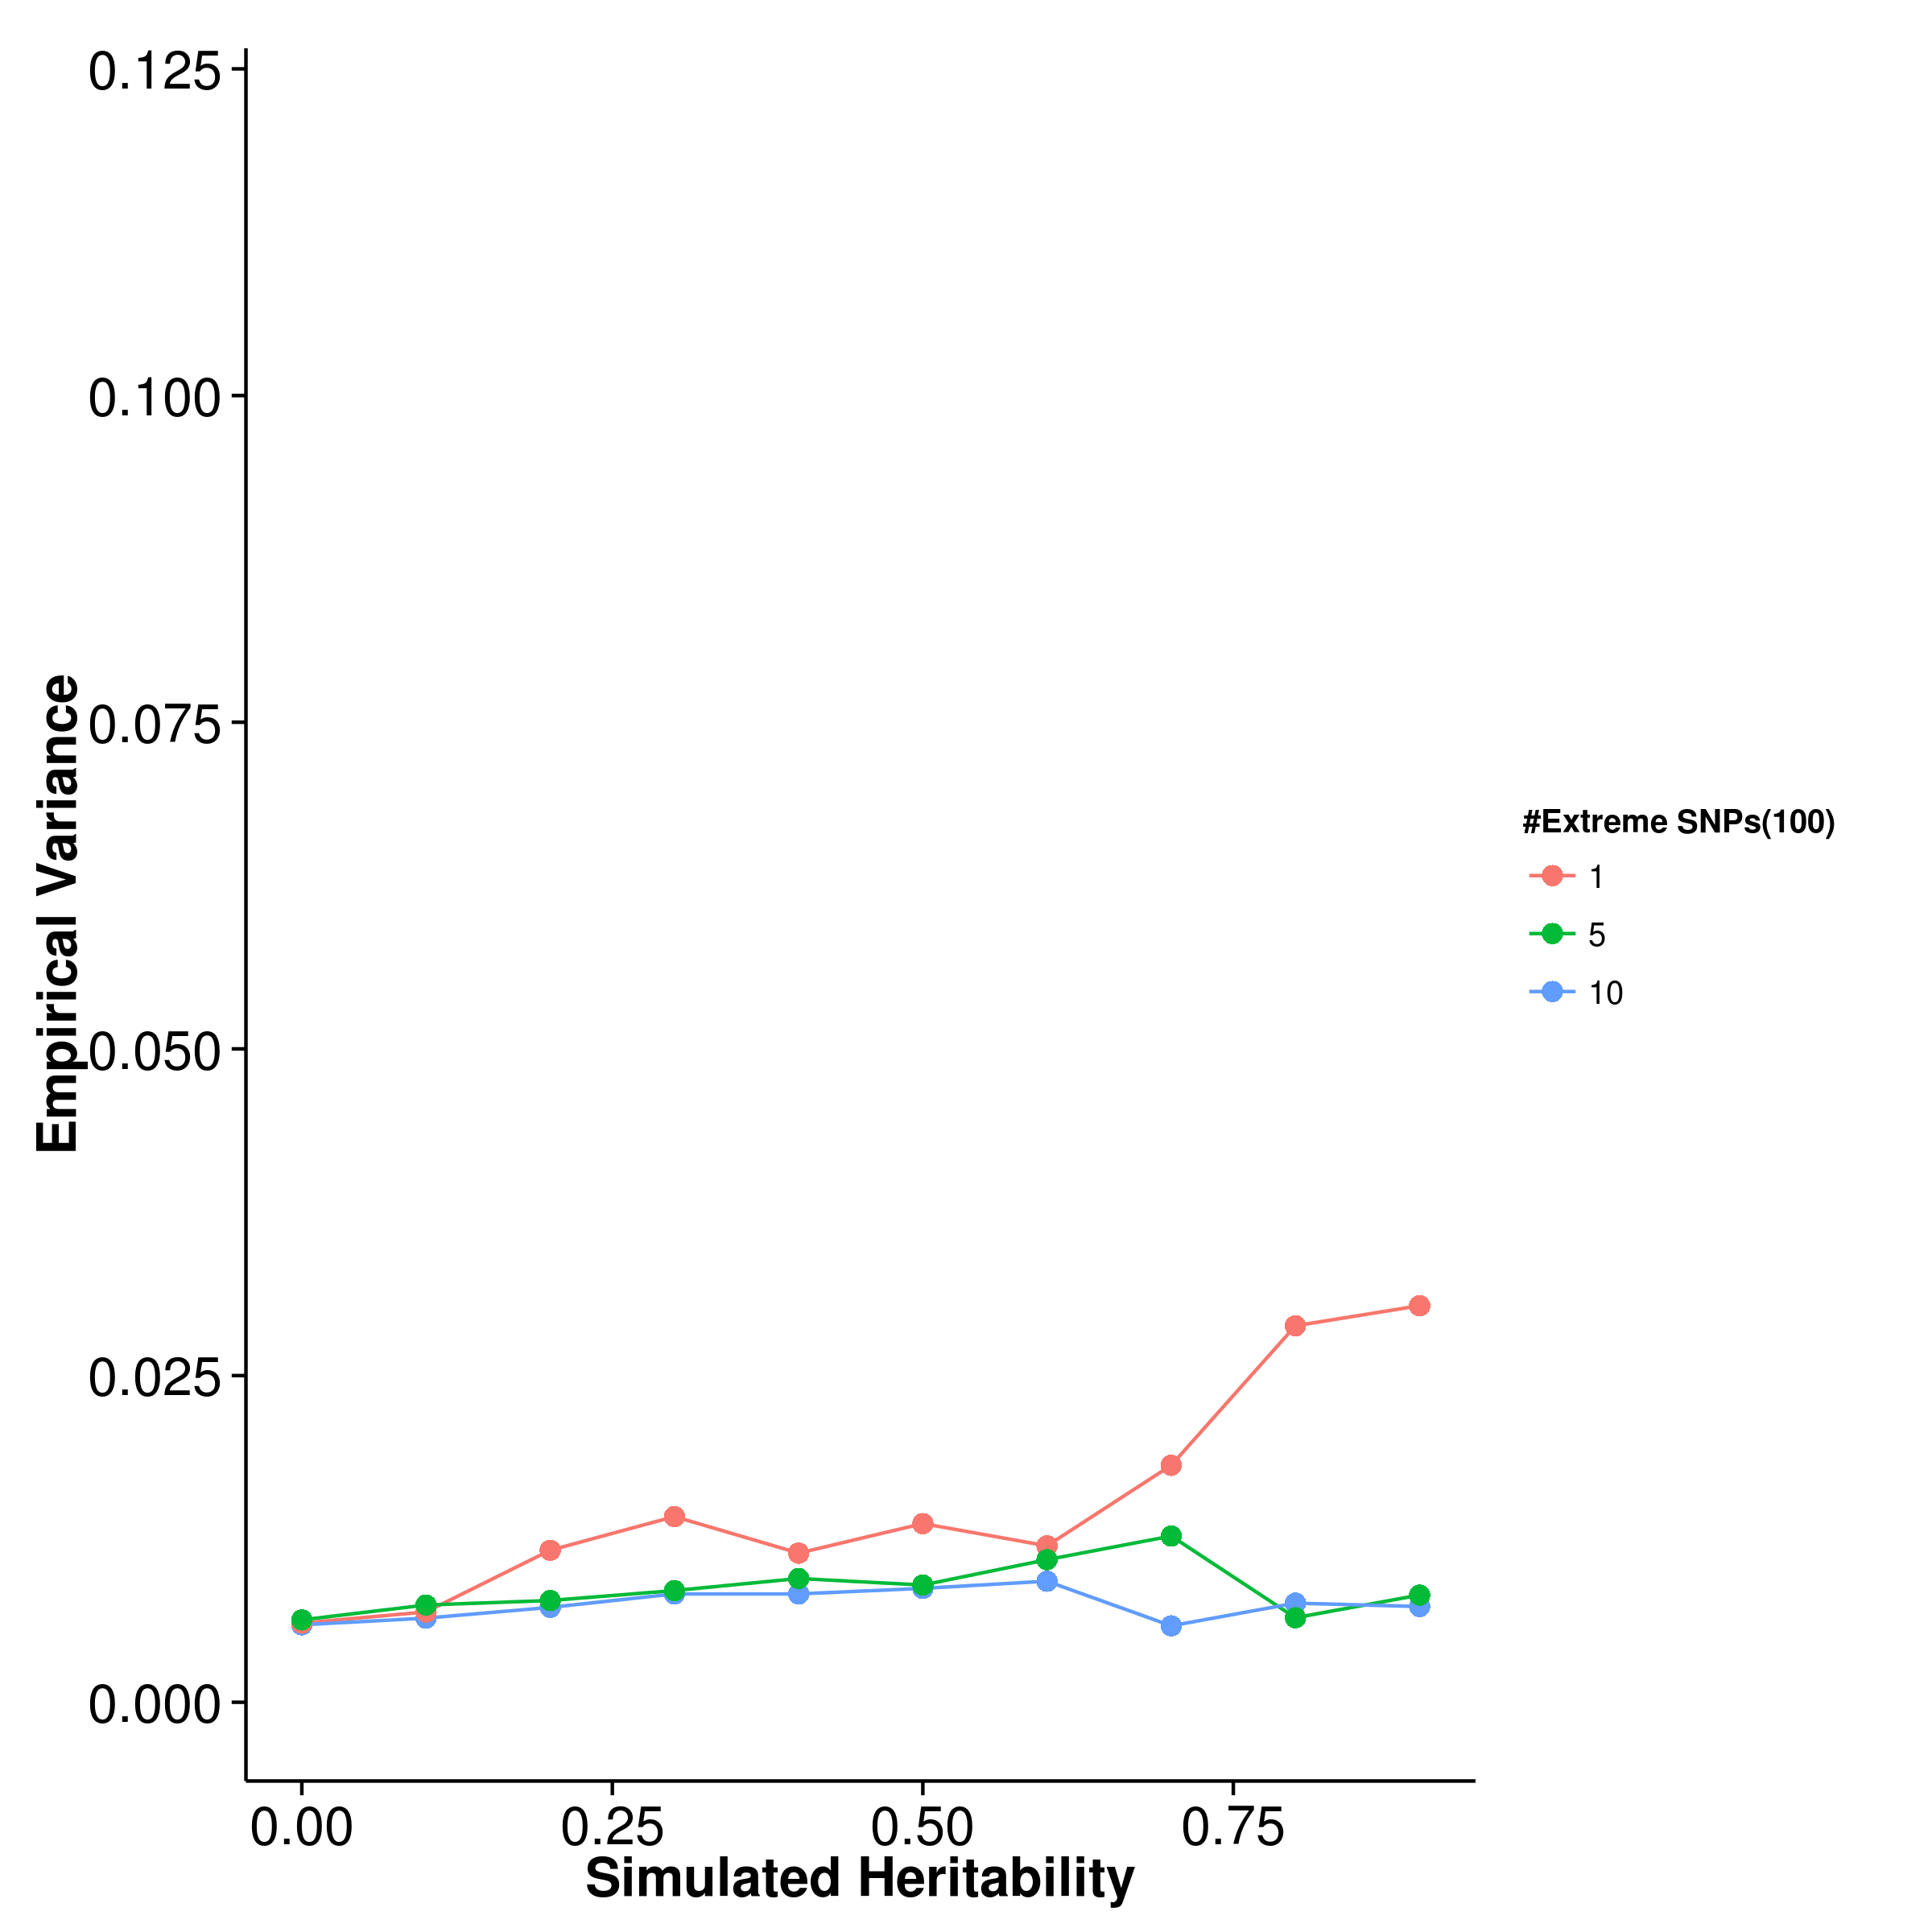
\includegraphics{figure/he_summary/extreme_100c/gcta_QtE_Extreme_sd.png}}
				\label{fig:gctaQtEx100cVar}
			}\\
			\subfloat[LDSC with fix intercept]{
				\scalebox{.4}{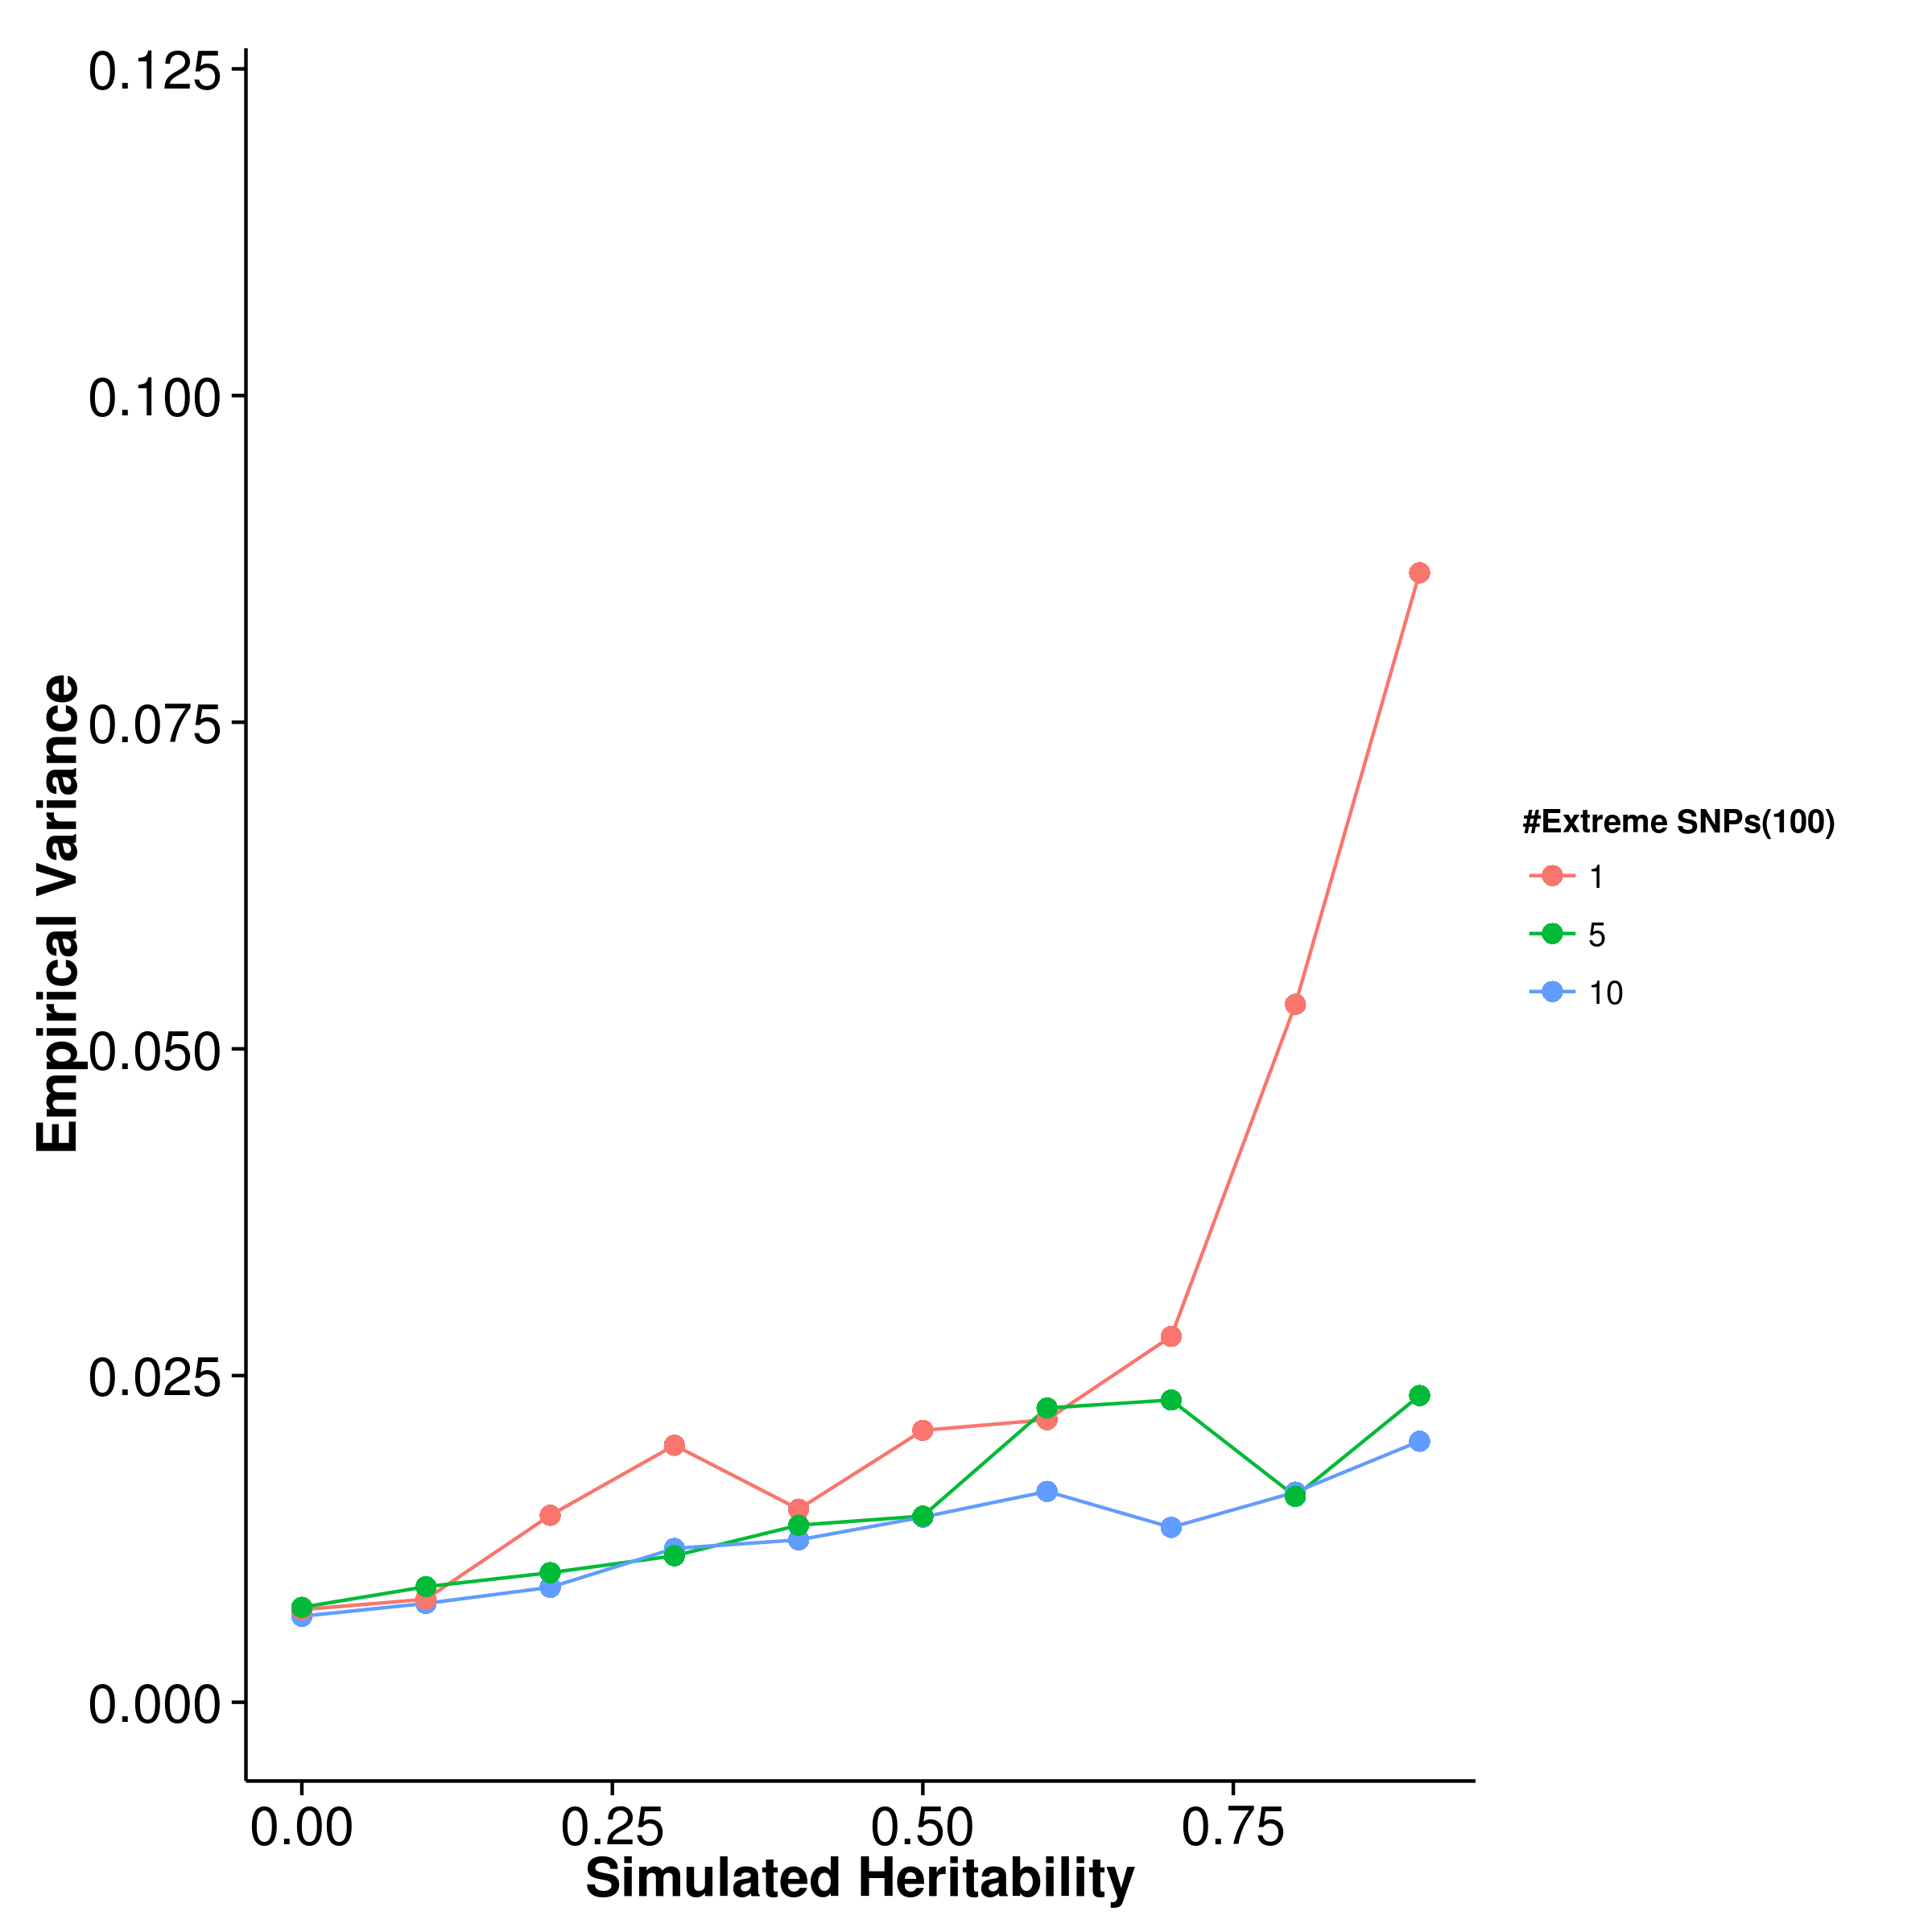
\includegraphics{figure/he_summary/extreme_100c/ldsc_QtE_Extreme_sd.png}}
				\label{fig:ldscQtEx100cVar}
			}
			\subfloat[LDSC with intercept estimation]{
				
				\scalebox{.4}{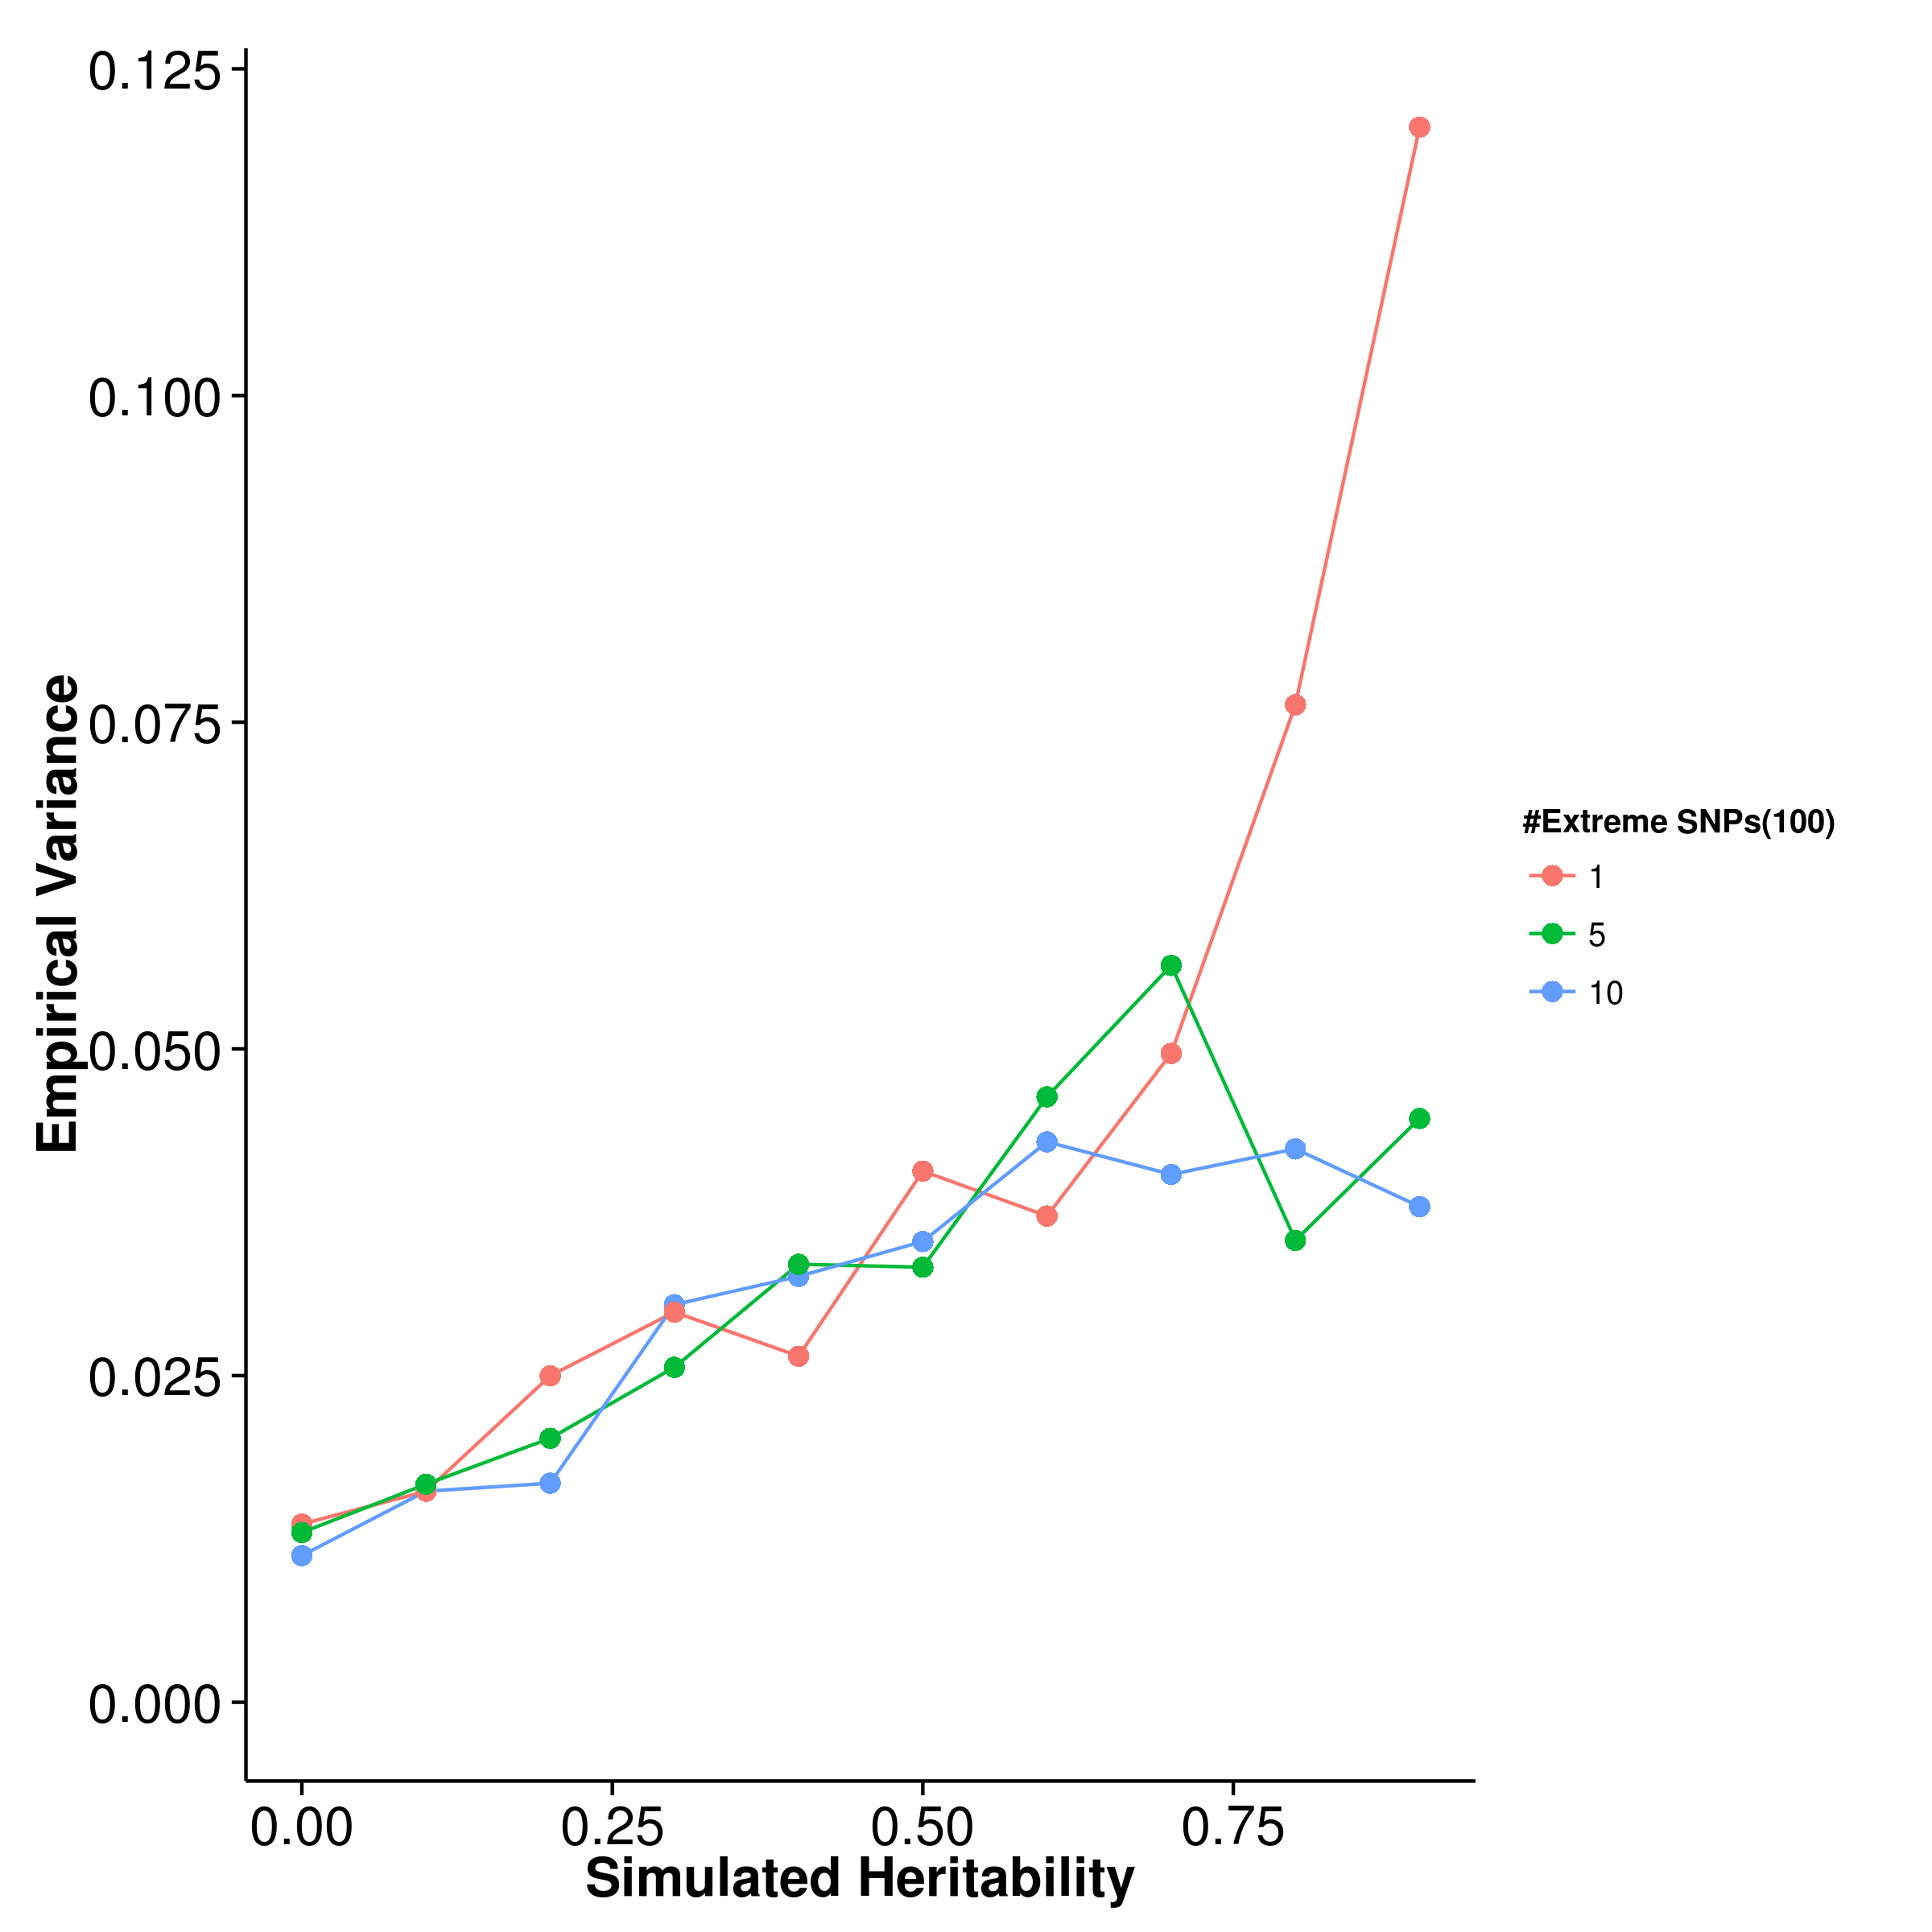
\includegraphics{figure/he_summary/extreme_100c/ldscIn_QtE_Extreme_sd.png}}
				\label{fig:ldscInQtEx100cVar}
			}
			\caption[Quantitative Trait with Extreme Effect Size Simulation Result(100 causal SNPs, Variance)]
			{Variance of results from quantitative trait simulation with extreme effect size simulation.
				100 causal \glspl{SNP} were simulated.
				\gls{gcta} has the smallest variance as with previous simulation.
				When compared to \gls{ldsc} with fixed intercept, although the variance of \gls{shrek} was relatively higher, it was less sensitive to change in heritability and the number of \glspl{SNP} explaining a large portion of effect.
				In situation where 1 \gls{SNP} represent 50\% of the effect, the variance of \gls{shrek} is actually lower than that of \gls{ldsc} with fixed intercept once the heritability was $\ge0.2$.
			} 
			\label{fig:QtEx100cVar}
		\end{figure}
		
		\begin{figure}
			\centering
			\subfloat[SHREK]{
				\scalebox{.4}{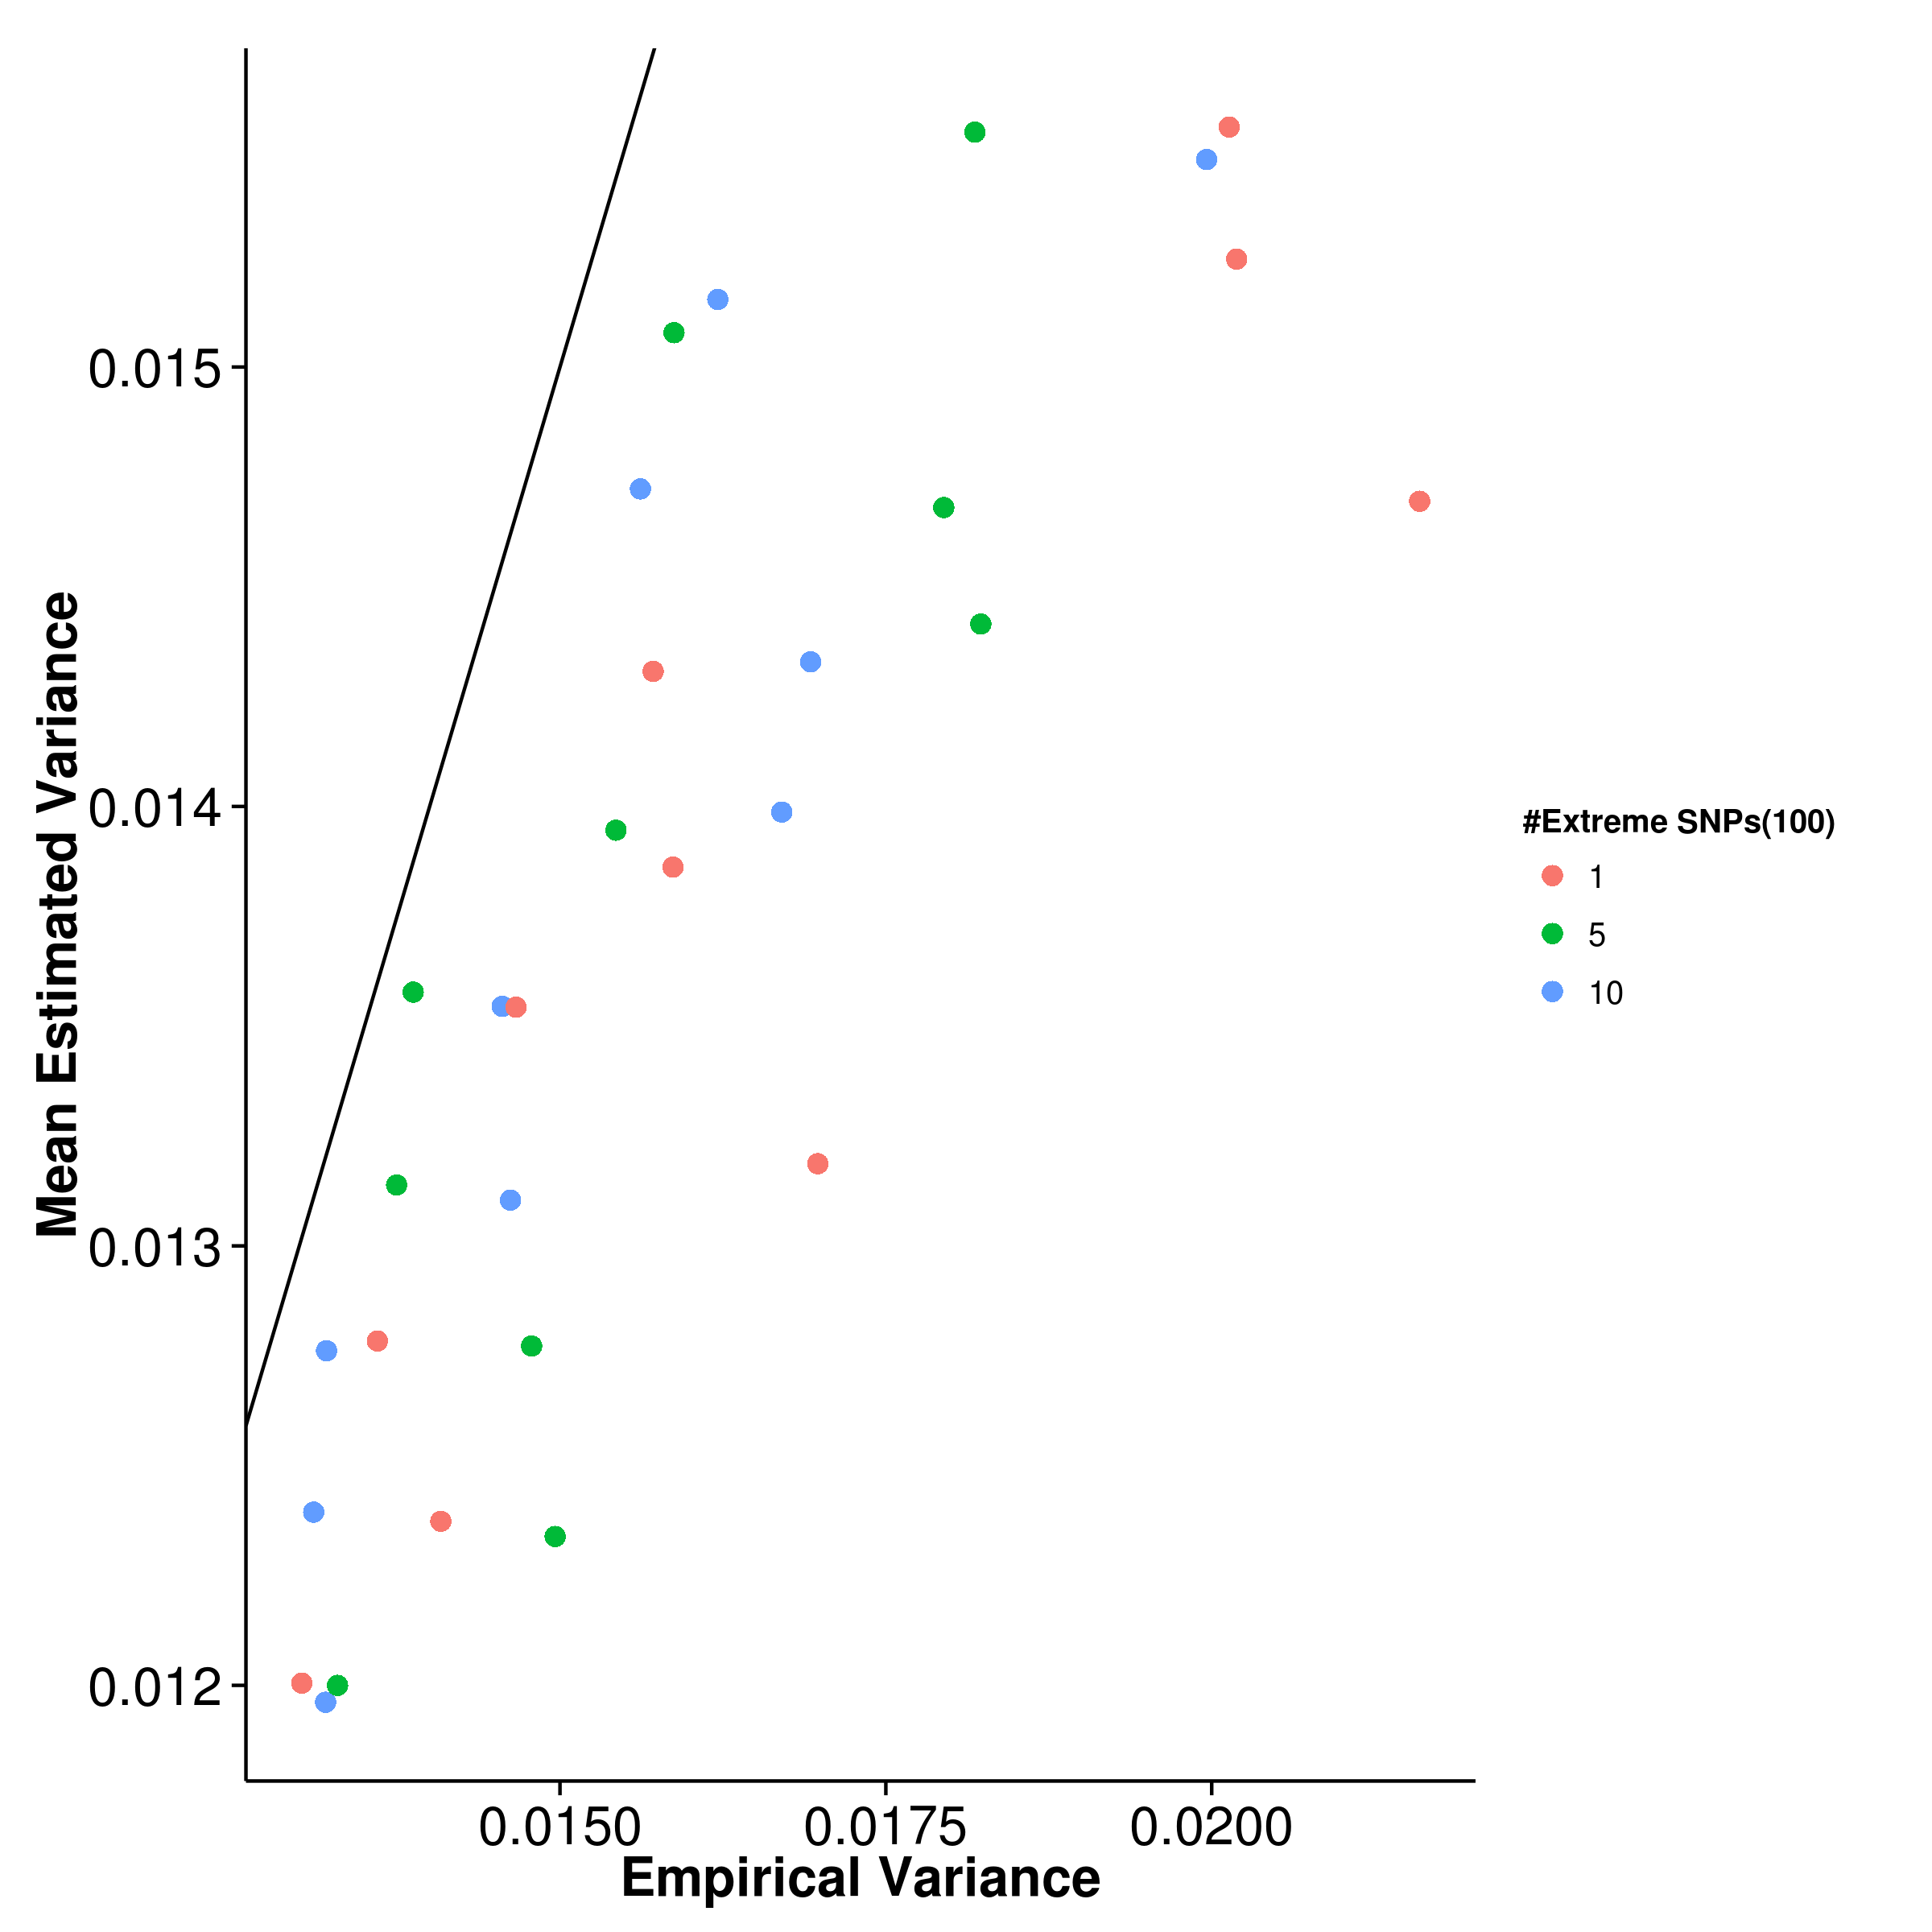
\includegraphics{figure/he_summary/extreme_100c/shrek_QtE_Extreme_sdCom.png}}
				\label{fig:shrekQtEx100cVarCom}
			}
			\subfloat[GCTA]{
				\scalebox{.4}{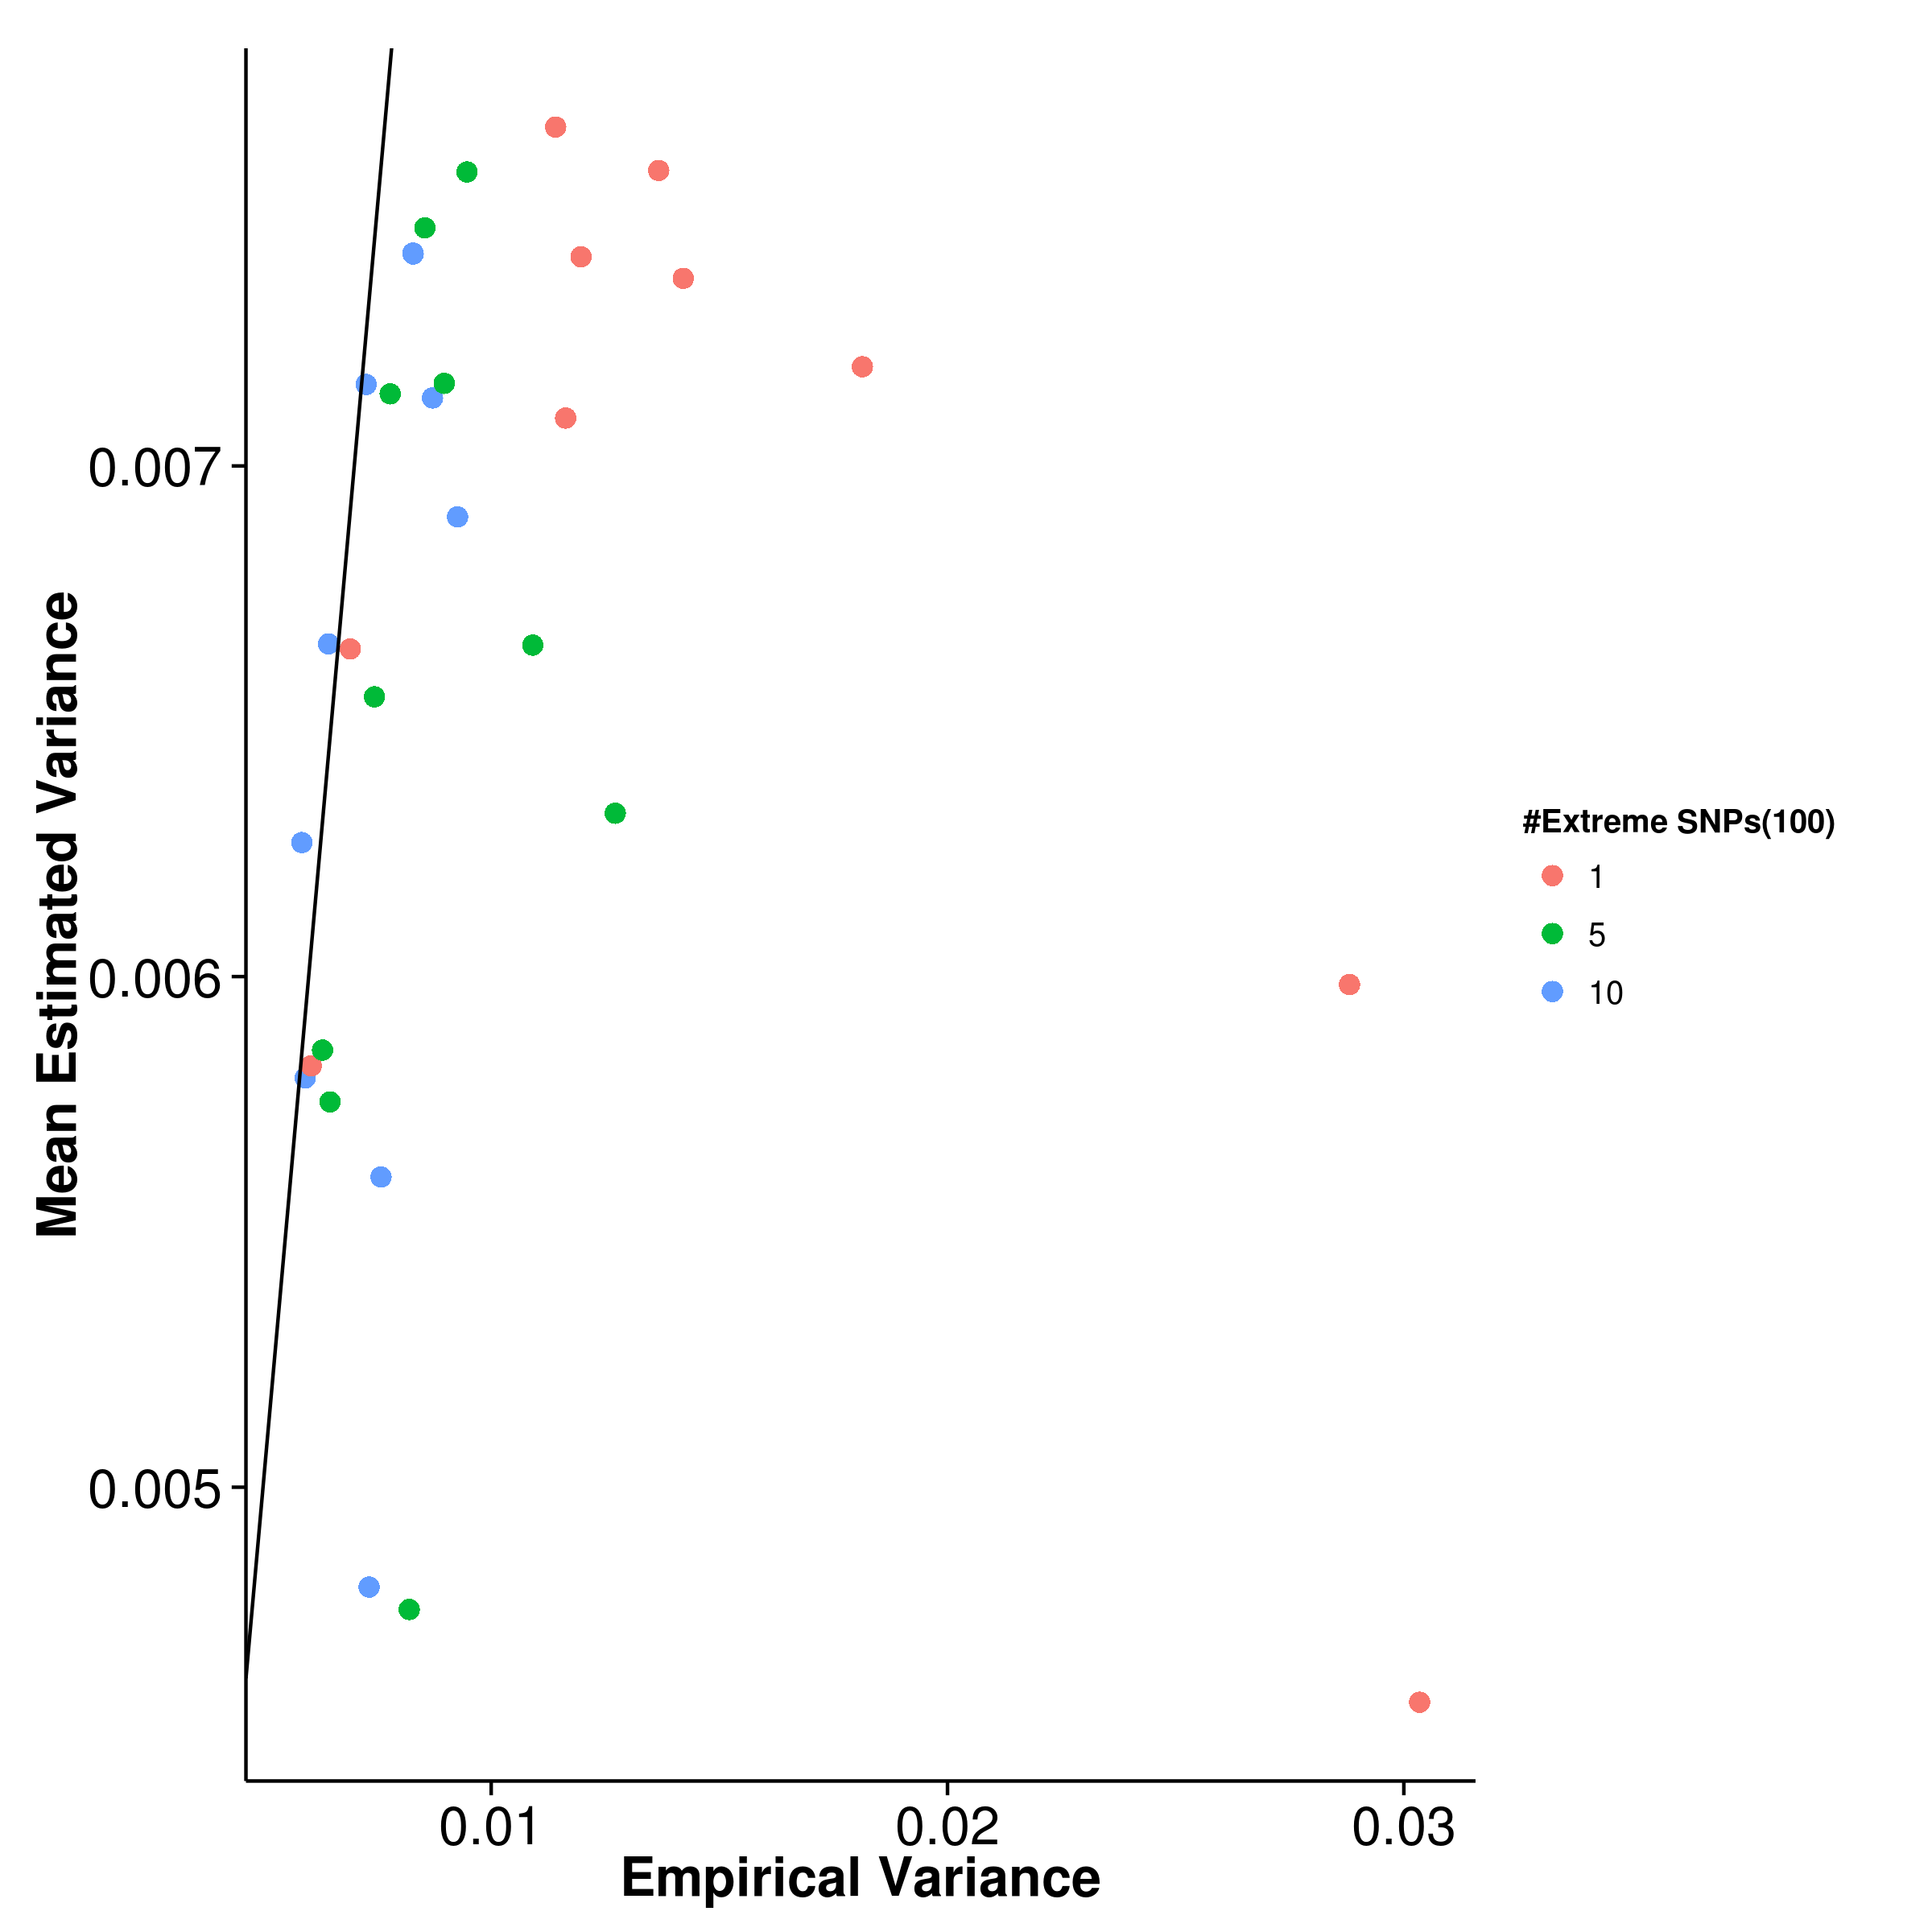
\includegraphics{figure/he_summary/extreme_100c/gcta_QtE_Extreme_sdCom.png}}
				\label{fig:gctaQtEx100cVarCom}
			}\\
			\subfloat[LDSC with fix intercept]{
				\scalebox{.4}{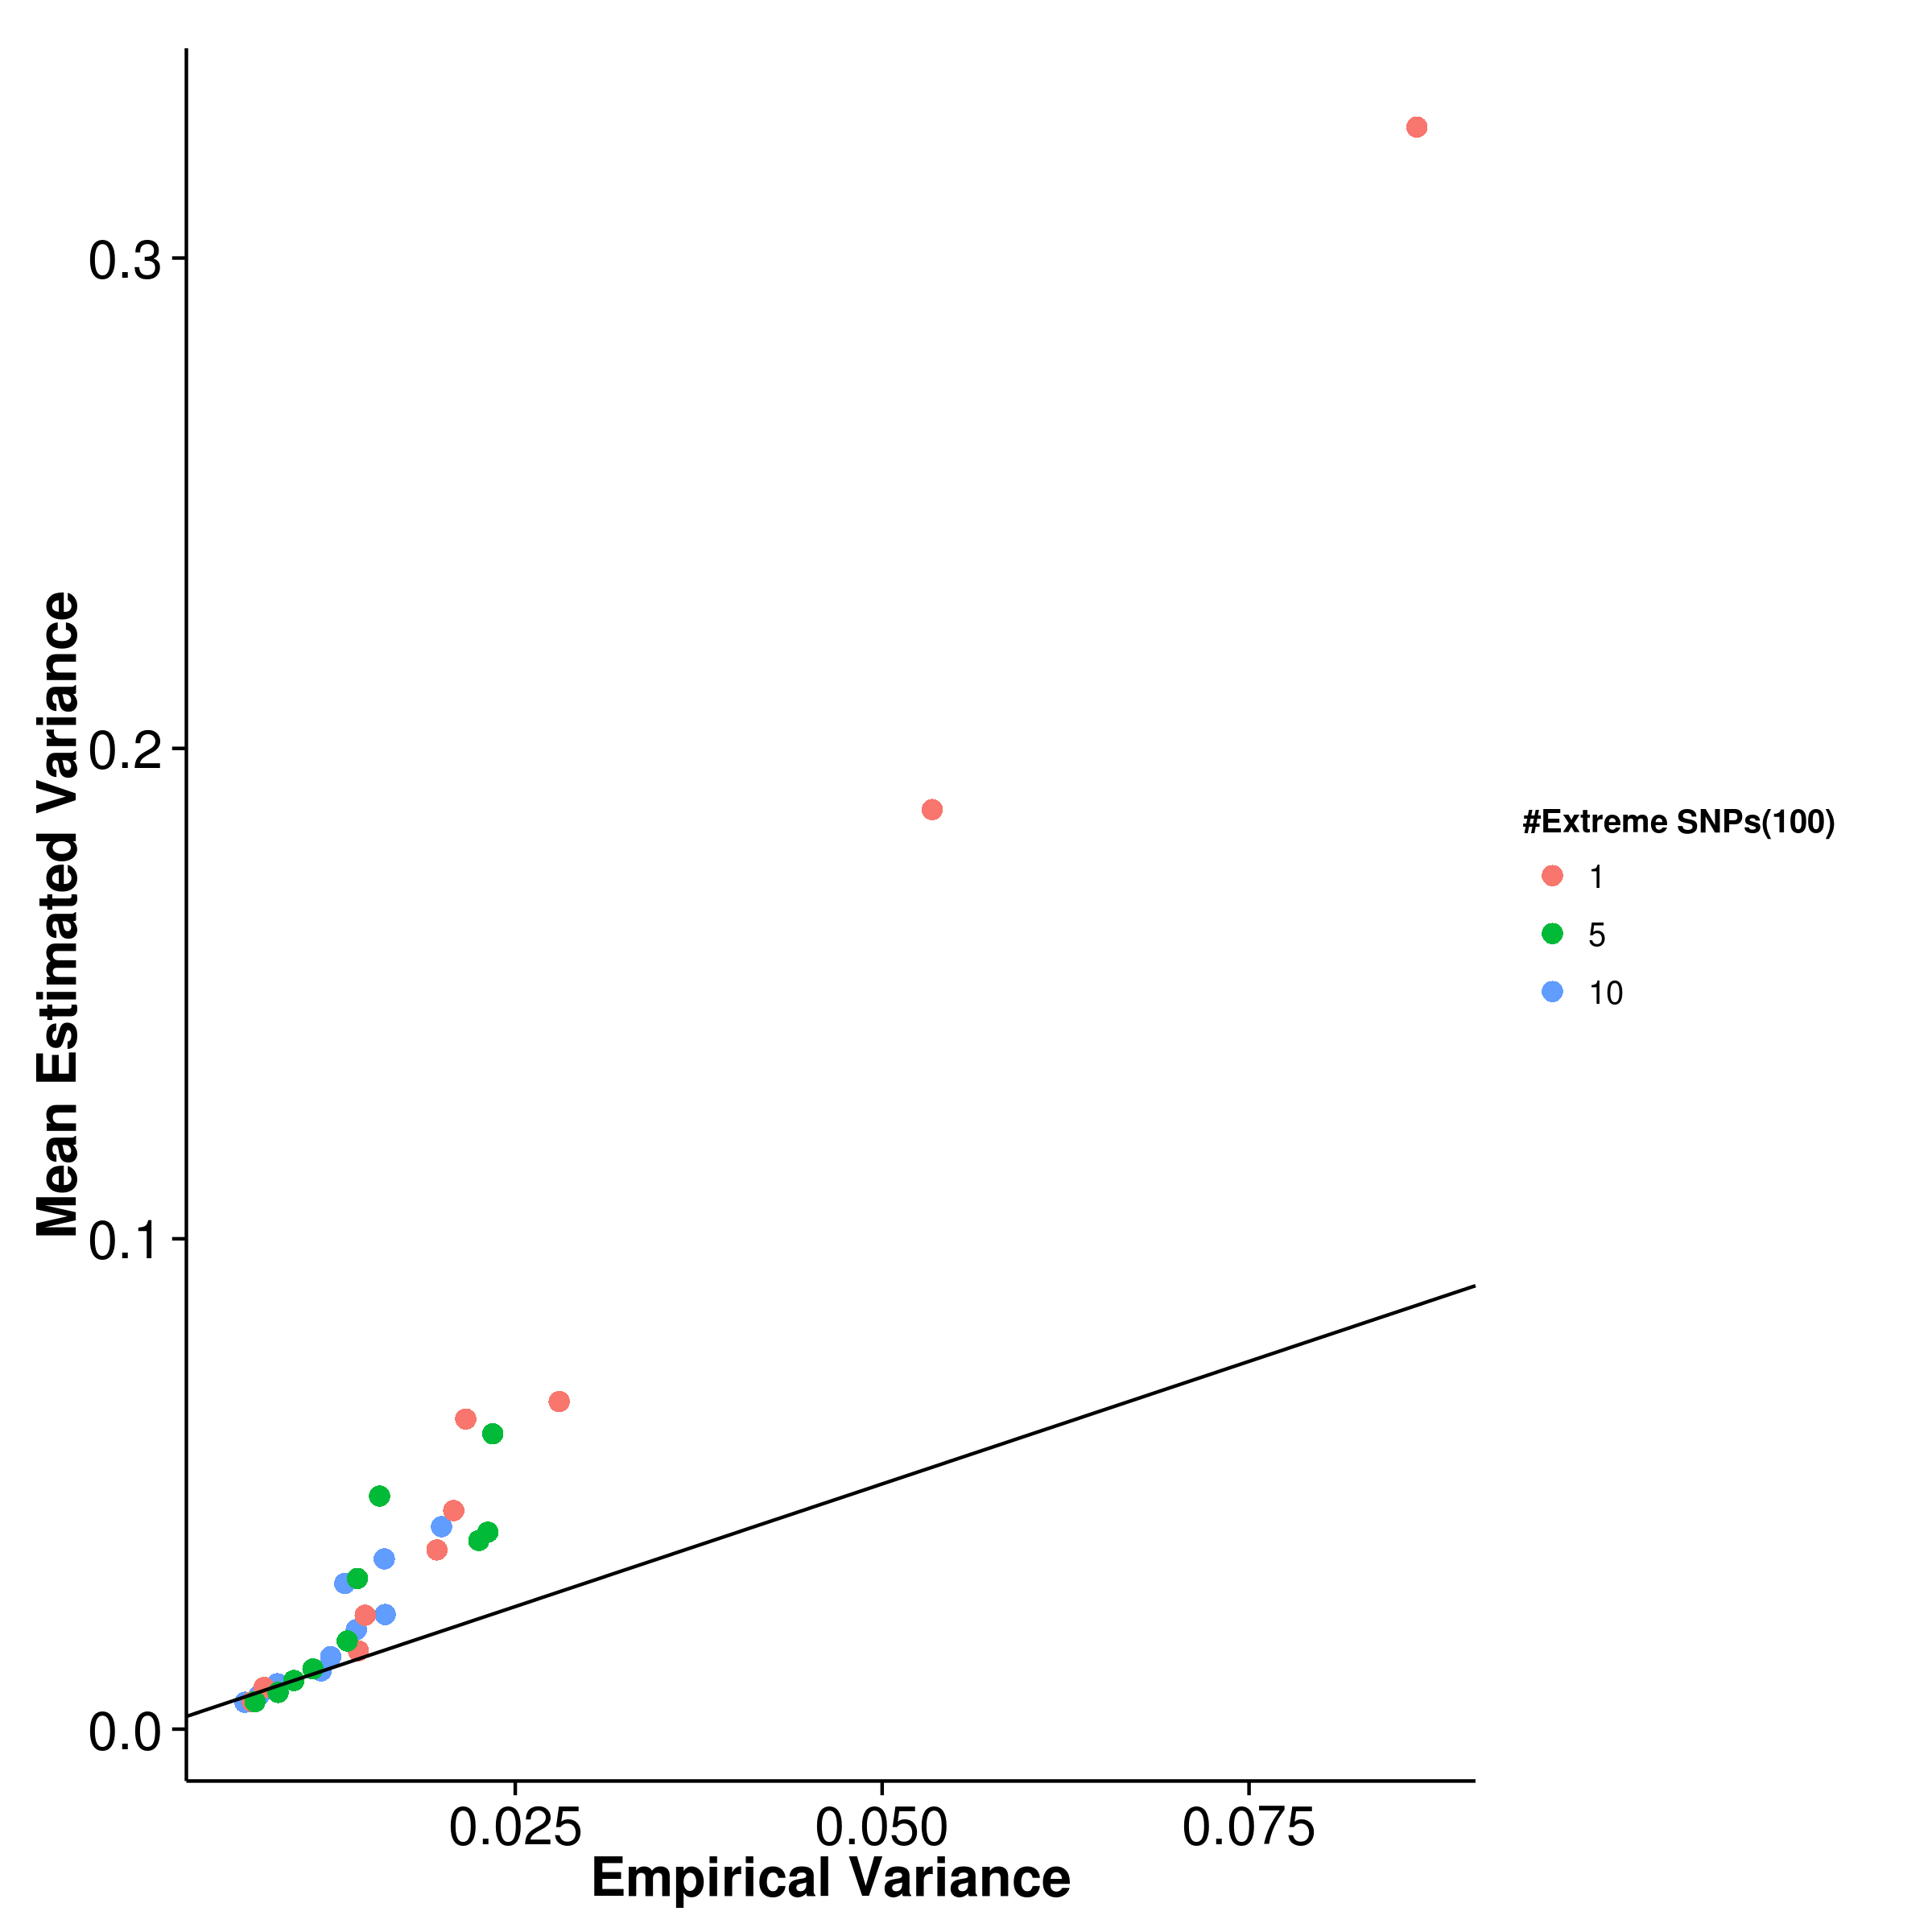
\includegraphics{figure/he_summary/extreme_100c/ldsc_QtE_Extreme_sdCom.png}}
				\label{fig:ldscQtEx100cVarCom}
			}
			\subfloat[LDSC with intercept estimation]{
				
				\scalebox{.4}{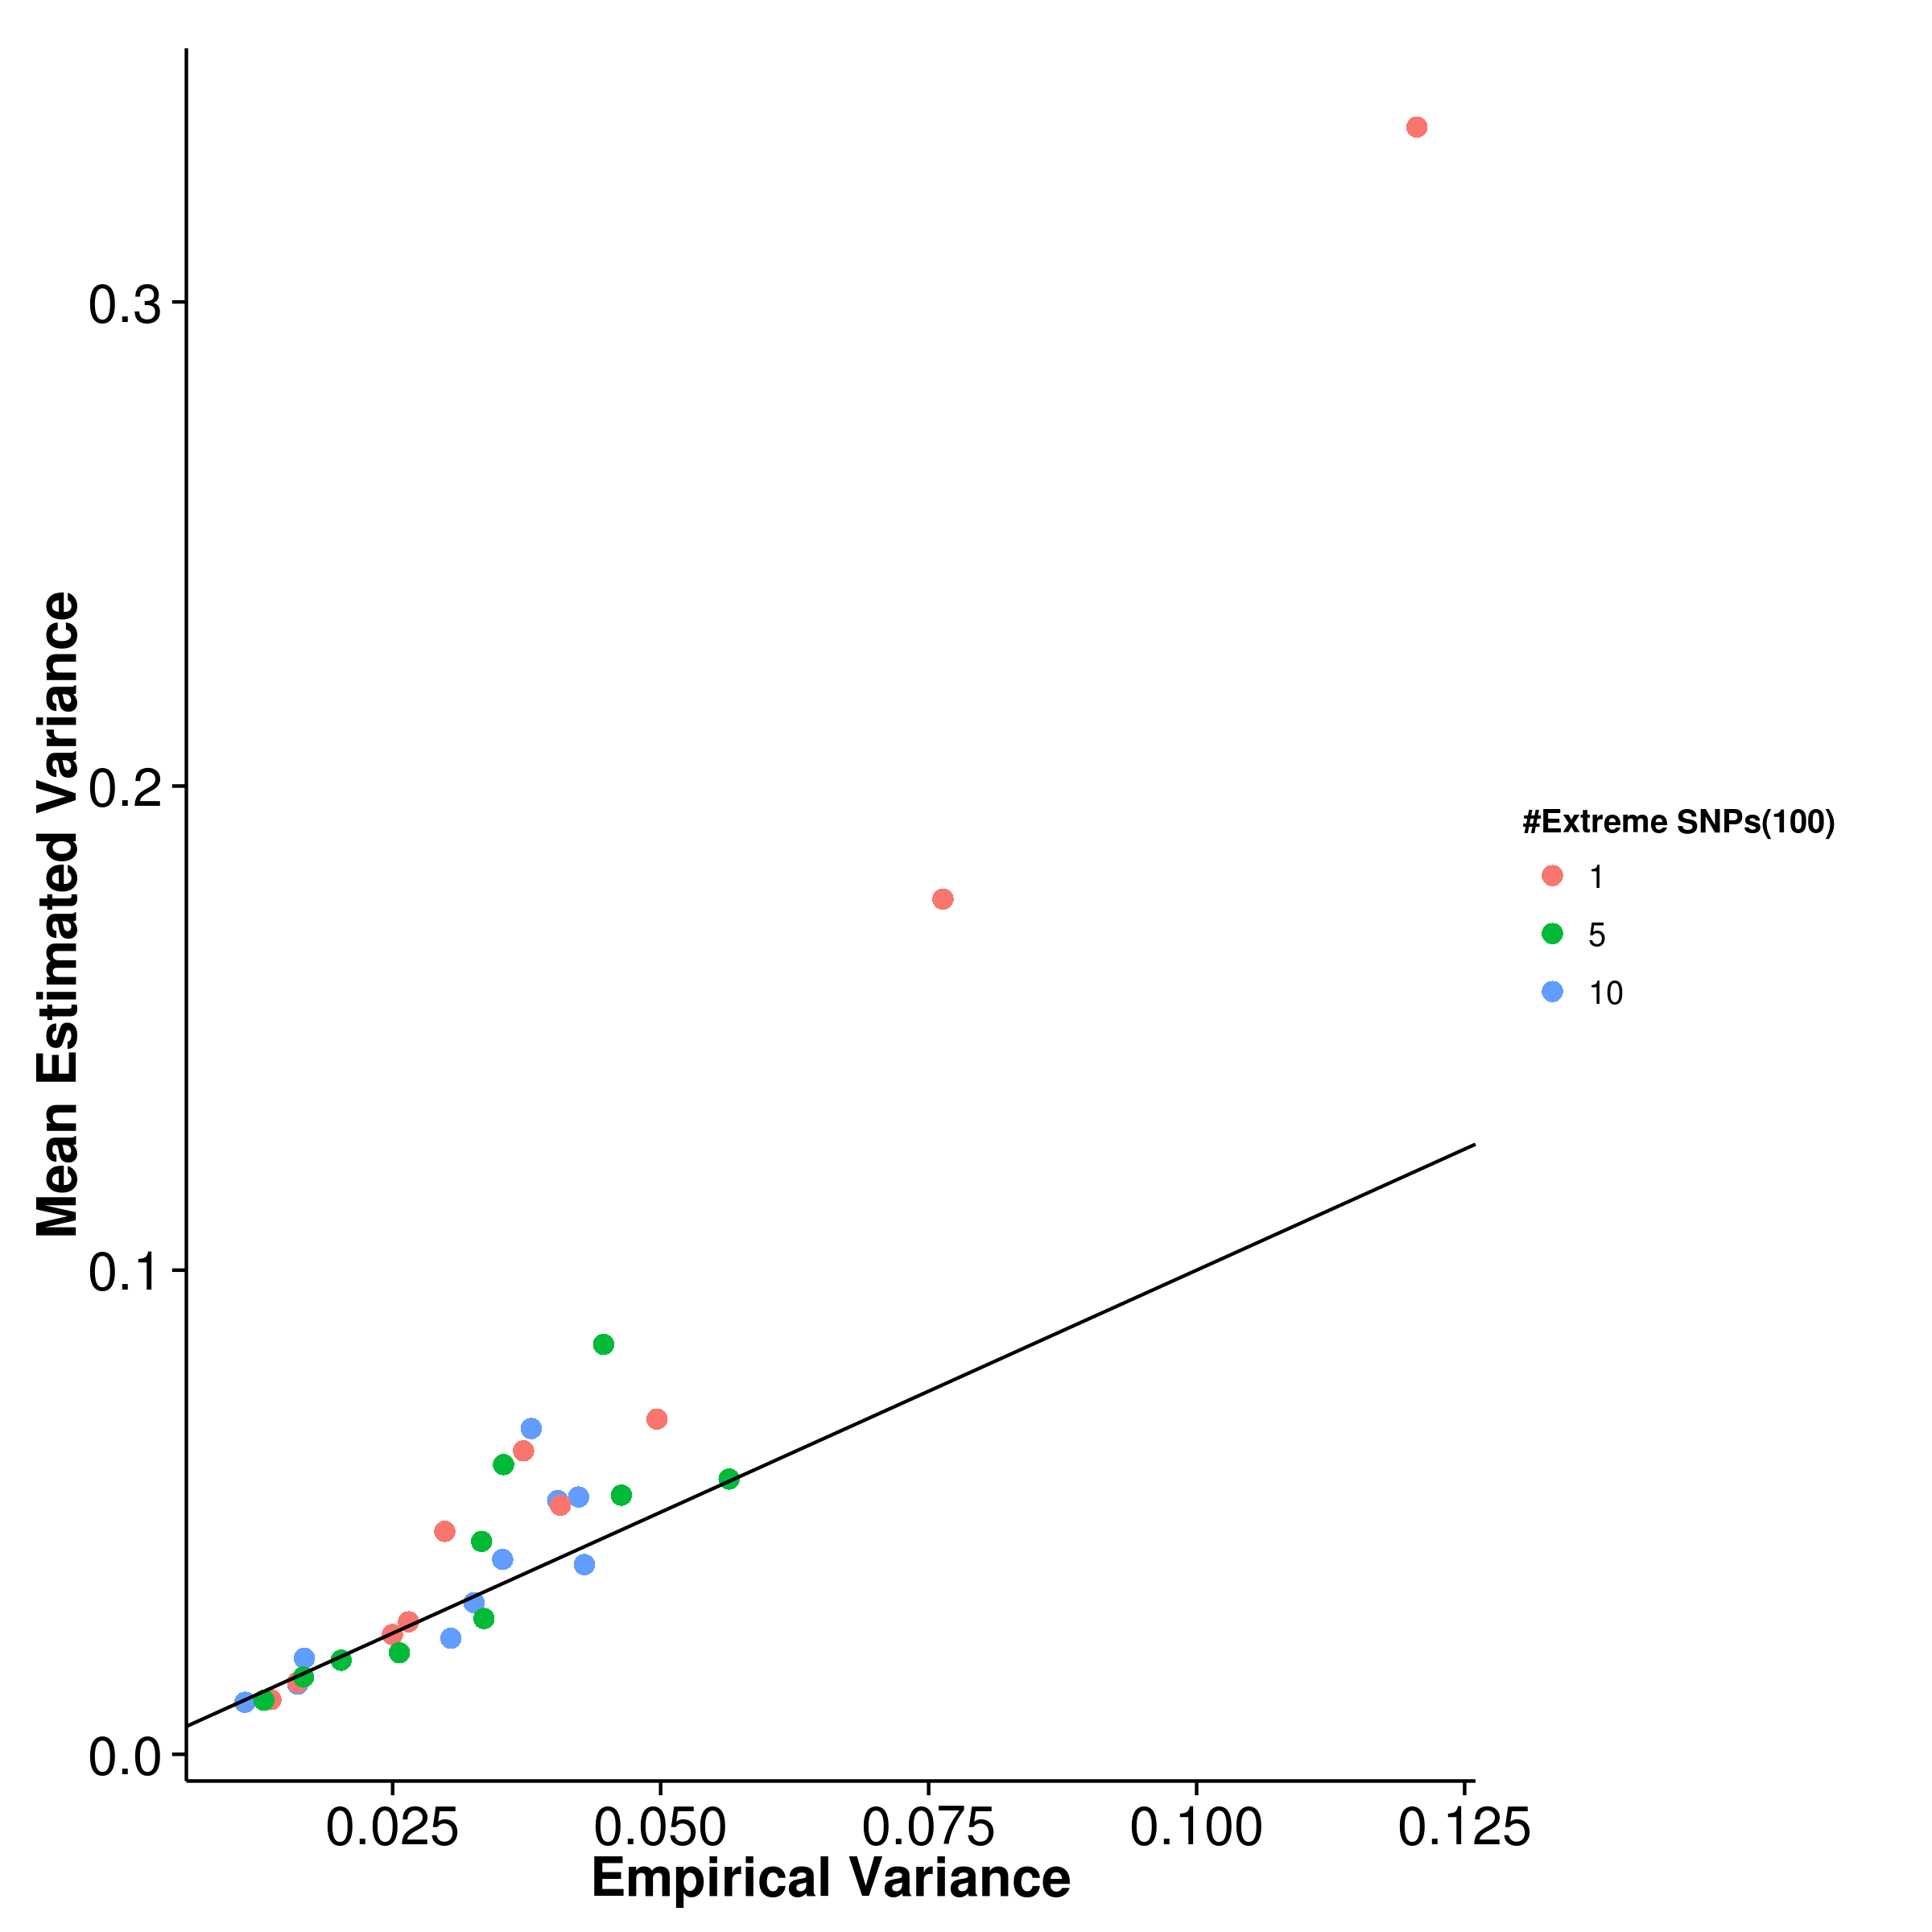
\includegraphics{figure/he_summary/extreme_100c/ldscIn_QtE_Extreme_sdCom.png}}
				\label{fig:ldscInQtEx100cVarCom}
			}
			\caption[Quantitative Trait with Extreme Effect Size Simulation Result(100 causal SNPs, Estimated Variance)]
			{Estimated variance of results from quantitative trait simulation with extreme effect size simulation when compared to the empirical variance.
				100 causal \glspl{SNP} were simulated.
				\gls{shrek} generally under-estimate the variance whereas \gls{ldsc} over-estimate the variance.
			} 
			\label{fig:QtEx100cVarCom}
		\end{figure}